\documentclass{article}
\usepackage{manualdoprofessor}
\usepackage{fichatecnica}
\usepackage{lipsum,media9,graficos}
\usepackage[justification=raggedright]{caption}
\usepackage{bncc}
\usepackage[kalinka]{logoedlab}
\usepackage{marginnote}

\begin{document}


\newcommand{\AutorLivro}{Daniela Mountian (Org.)}
\newcommand{\TituloLivro}{Contos russos infanto juvenis}
\newcommand{\Tema}{Ficção, mistério e fantasia}
\newcommand{\Genero}{Conto, crônica e novela}
% \newcommand{\imagemCapa}{PNLD0050-01.png}
\newcommand{\issnppub}{---}
\newcommand{\issnepub}{---}
% \newcommand{\fichacatalografica}{PNLD0050-00.png}
\newcommand{\colaborador}{\textbf{Marina Darmaros} é uma pessoa incrível e vai fazer um bom serviço.}


\title{\TituloLivro}
\author{\AutorLivro}
\def\authornotes{\colaborador}

\date{}
\maketitle
\tableofcontents

\pagebreak

\section{Carta aos professores}

Caro educador / Cara educadora,\\\bigskip

O presente manual tem por objetivo oferecer apoio pedagógico àqueles
para quem o livro \emph{Contos russos} \emph{juvenis} foi pensado e
preparado: educandos do ensino médio. A pessoa fundamental para o
sucesso desse encontro é justamente você, que educa, a quem convidamos a
mergulhar nas fascinantes histórias de alguns dos maiores autores russos
de todos os tempos.

A coletânea traz quinze contos, de 1781 até 1928, em traduções feitas
diretamente do russo para o português. Queremos apresentar a literatura
clássica russa destinada ao público jovem, dando uma amostragem vasta de
temas e estilos. Buscamos também ampliar o repertório de clássicos
juventude com obras que dão ao leitor de entrar em contato com uma
cultura rica e completamente diferente da dele, o que alargará a
percepção que ele tem de si e do mundo. O volume tem uma lógica interna,
ou seja, contém contos que se ligam entre si, e também marca pontos
importantes do desenvolvimento das letras clássicas russas juvenis até o
início do século \textsc{xx}.

Além de reunir linguagens e gêneros diferentes, os contos revelam
questões literárias, sociais e históricas que serão contextualizadas e
aprofundadas nas atividades aqui propostas, as quais incentivarão a
pesquisa, a produção de textos e o desenvolvimento de outras
multimodalidades. O intuito deste manual é, no fim das contas, ajudar a
tornar a leitura um hábito e um prazer na vida d jovens do ensino médio.

Esperamos que achem este material proveitoso para o trabalho em sala de
aula!


\section{Atividades 1}

\BNCC{EM13LP01}
\BNCC{EM13LP46}
\BNCC{EM13LP49}

Orientações para as aulas de Língua Portuguesa, a fim de preparar
os educandos para a leitura da obra (seção Pré"-leitura), assim como para
sua análise e problematização (Pós"-leitura).

\paragraph{Tema} ``O pescador de momentos'': introduzindo a leitura e o gênero do conto.

\paragraph{Conteúdo}
Apresentação, leitura e compreensão de alguns dos \emph{Contos russos
juvenis} e do gênero do conto em si. Trazemos algumas sugestões, mas o
educador pode selecionar os textos que considerar mais pertinentes para
a atividade.

\paragraph{Objetivos}
Ajudar o jovem leitor a se familiarizar com o gênero do conto, uma das
mais efetivas formas de expressão no letramento literário.

\paragraph{Justificativa}
A experiência direta com o conto como gênero textual é uma maneira muito
eficaz de incentivar o gosto pela leitura. Conciso e encerrando em si um
rigoroso trabalho de seleção, até mesmo devido à extensão limitada, o
conto normalmente tem grande apelo ao trazer um episódio singular ou
representativo e um número restrito de personagens.

Nesta coletânea, são apresentados quinze contos, de 1781 a 1928, de
renomados escritores russos, com grande variedade de temas e estilos Há
desde textos de linguagem realista e de denúncia, buscando despertar no
jovem preocupação e consciência social, até obras do séc. \textsc{xx} que mostram
a transformação da ideia de infância, que agora se expressa em universos
lúdicos, incentivando a imaginação e a brincadeira or exemplo, em ``A
pedrinha vermelha'' (1911), Sacha Tchórny ``traz o olhar e a
lógica adorável da criança e os leva para o plano da linguagem''
(\textsc{mountian}, 2021, p. 25); em ``Sobre como Kolka Pánkin viajou para o
Brasil e sobre como Pietka Erchóv não acreditou em nada'' (1928), Daniil
Kharms, que trabalhando elementos do \emph{nonsense}, apresenta um conto
, sem didatismos.

\paragraph{Metodologia}
O educador pode iniciar uma leitura coletiva para apresentar o texto
escolhido e mostrar sua acessibilidade aos educandos. A recomendação,
porém, é que a leitura coletiva abarque um conto completo e não apenas
trechos. Seguem alguns pontos que podem ser selecionados para esta
atividade:

\subsection{Pré"-leitura}

\paragraph{Tema} Pensando no conto.

É interessante, nesta fase, explicar ao aluno um pouco sobre o gênero
literário com que ele trabalhará, destacando alguns pontos"-chaves, tais
como:

O conto é uma narrativa centrada em um fato ou acontecimento, com uma
unidade dramática e se mistura ``aos primórdios da própria arte
literária''. (\textsc{moisés}, 2004, p. 87) Recebeu várias acepções ao longo dos
séculos; passou por lendas orientais, parábolas bíblicas, novelas
medievais italianas, fábulas francesas até chegar ao século \textsc{xix} e ganhar
\emph{status} literário próprio.

Questões sugeridas: Alguém se recorda de algum autor de contos? Tem
algum conto favorito? Pode falar sobre ele à sala?

O conto difere do romance e da novela não só pela extensão, mas por
ter uma estrutura própria: ele registra de forma literária um episódio
singular ou representativo, sem buscar abarcar a totalidade, mas, sim,
uma amostra da realidade ou um flagrante. É uma narrativa concisa, de
poucas personagens, delineando apenas uma história, um conflito. Como
ironizou Cortázar, parafraseando um amigo, nesse combate similar ao do
boxe, ``o romance ganha sempre por pontos, enquanto o conto deve ganhar
por nocaute''. Já Bosi poetiza (1973, p. 9), ``Em face da história, rio
sem fim que vai arrastando tudo e todos no seu curso, o contista é um
pescador de momentos singulares cheios de significação''.

Uma proposta é que o estudante faça uma pesquisa prévia, pela internet
ou na biblioteca, sobre o conto como gênero e alguns de seus expoentes.
Cabe também pedir ao estudante que busque a diferença entre o conto
literário e o popular, folclórico ou fantástico, ``como os de Grimm ou
Perrault, ainda caracterizados pela oralidade. Estes, de criação
espontânea, fazem parte do que André Jolles chamou de `formas
simples'''. (\textsc{soares}, 2007, p. 55)

\subsection{Leitura}

Cada conto poderá ser lido individualmente para discussão em aula, mas a
leitura coletiva é o caminho que recomendamos para a aproximação inicial
dos educandos e os textos, de modo que sejam incentivados a relê"-los.
Fornecemos a seguir uma proposta de leitura que abarca dois pontos
extremos da coletânea: 1) ``Conto do tsarévitche Cloro'' (1781), um dos
primeiros textos em prosa para crianças, escrito por Catarina, a Grande,
soberana célebre que incentivou as letras e as artes, e 2) ``Sobre como
Kolka Pánkin viajou para o Brasil e sobre como Pietka Erchóv não
acreditou em nada'' (1928), de Daniil Kharms, que se tornou um dos
expoentes da literatura infantojuvenil no país nos anos 1920.

\begin{enumerate}
\item ``Conto do Tsarévitche Cloro'' (1781)
\end{enumerate}

\reversemarginpar
\marginparwidth=5cm

\marginnote{\footnotesize \textbf{PARA LER}\\
\emph{Recontar o tempo: apresentação e tradução da
Narrativa dos anos passados}. Tese de doutorado (\textsc{usp}) de Lucas Simone
sobre a Rus Kievana que pode fundamentar o conhecimento do período e
jogar luz sobre a ideia de tempo histórico pretendida por Catarina neste
conto.\\
\url{https://teses.usp.br/teses/disponiveis/8/8155/tde-21082019-115908/pt-br.php}
}

A literatura russa infantil se consolidou no romantismo, mas teve um
avanço importante na segunda metade do século \textsc{xviii}, no reinado de
Catarina \textsc{ii} (1729--1796), como visto no prefácio do livro. Naquela
época, a aristocracia se recusava a falar russo (os nobres, em geral, se
comunicavam em francês) e a população não era alfabetizada, por isso a
maior parte das publicações literárias para a infância ainda era
composta por títulos estrangeiros. Catarina é considerada pioneira na
prosa literária infantojuvenil russa por dois textos, e um deles é o
``Conto do tsarévitche Cloro'', que dedicou aos netos, Alexandre, futuro
imperador, e Constantino.

``Conto do tsarévitche Cloro'', que introduz a coletânea,
relata a trajetória do filho de um tsar bondoso e justo. Um dia, os pais
do tsarévitche Cloro o deixam com sete babás e partem para defender o
reino. É quando um cã quirguiz fica sabendo da beleza e da inteligência
de Cloro, atrai o menino e o leva para seu reino. Para se libertar de
lá, o tsarévitche precisa, segundo as ordens do cã, encontrar ``uma rosa
sem espinhos, que não pique''. Guiado pelo neto do cã, Juízo, que lhe
mostra o ``caminho reto'', o tsarévitche inicia sua jornada.


Se hoje a imaginação e a liberdade são normalmente estimuladas nos
livros para crianças e jovens, antes os contos destinados a eles eram
mais edificantes e didáticos, e esa parábola de Catarina, a Grande, é
exemplo disso. A parábola é um texto curto e de estrutura simples que
evidencia questões éticas e morais. Ela dialoga com a fábula, mas nesta
são os animais que virtudes morais, enquanto são as pessoas que o fazem
na parábola --- definida por Massaud Moisés como: ``Narrativa curta, não
raro identificada com o apólogo e a fábula, em razão da moral, explícita
ou implícita, que encerra, e da sua estrutura dramática. Todavia,
distingue"-se das outras duas formas literárias pelo fato de ser
protagonizada por seres humanos.'' (\textsc{moisés}, 2004, p. 337)

Questões sugeridas: Sabem o que é uma parábola? Quais elementos éticos e
morais foram destacados pela imperatriz? São elementos atemporais? A
obra tem caráter moralizador? As personagens são desenvolvidas?

\begin{figure}[ht!]
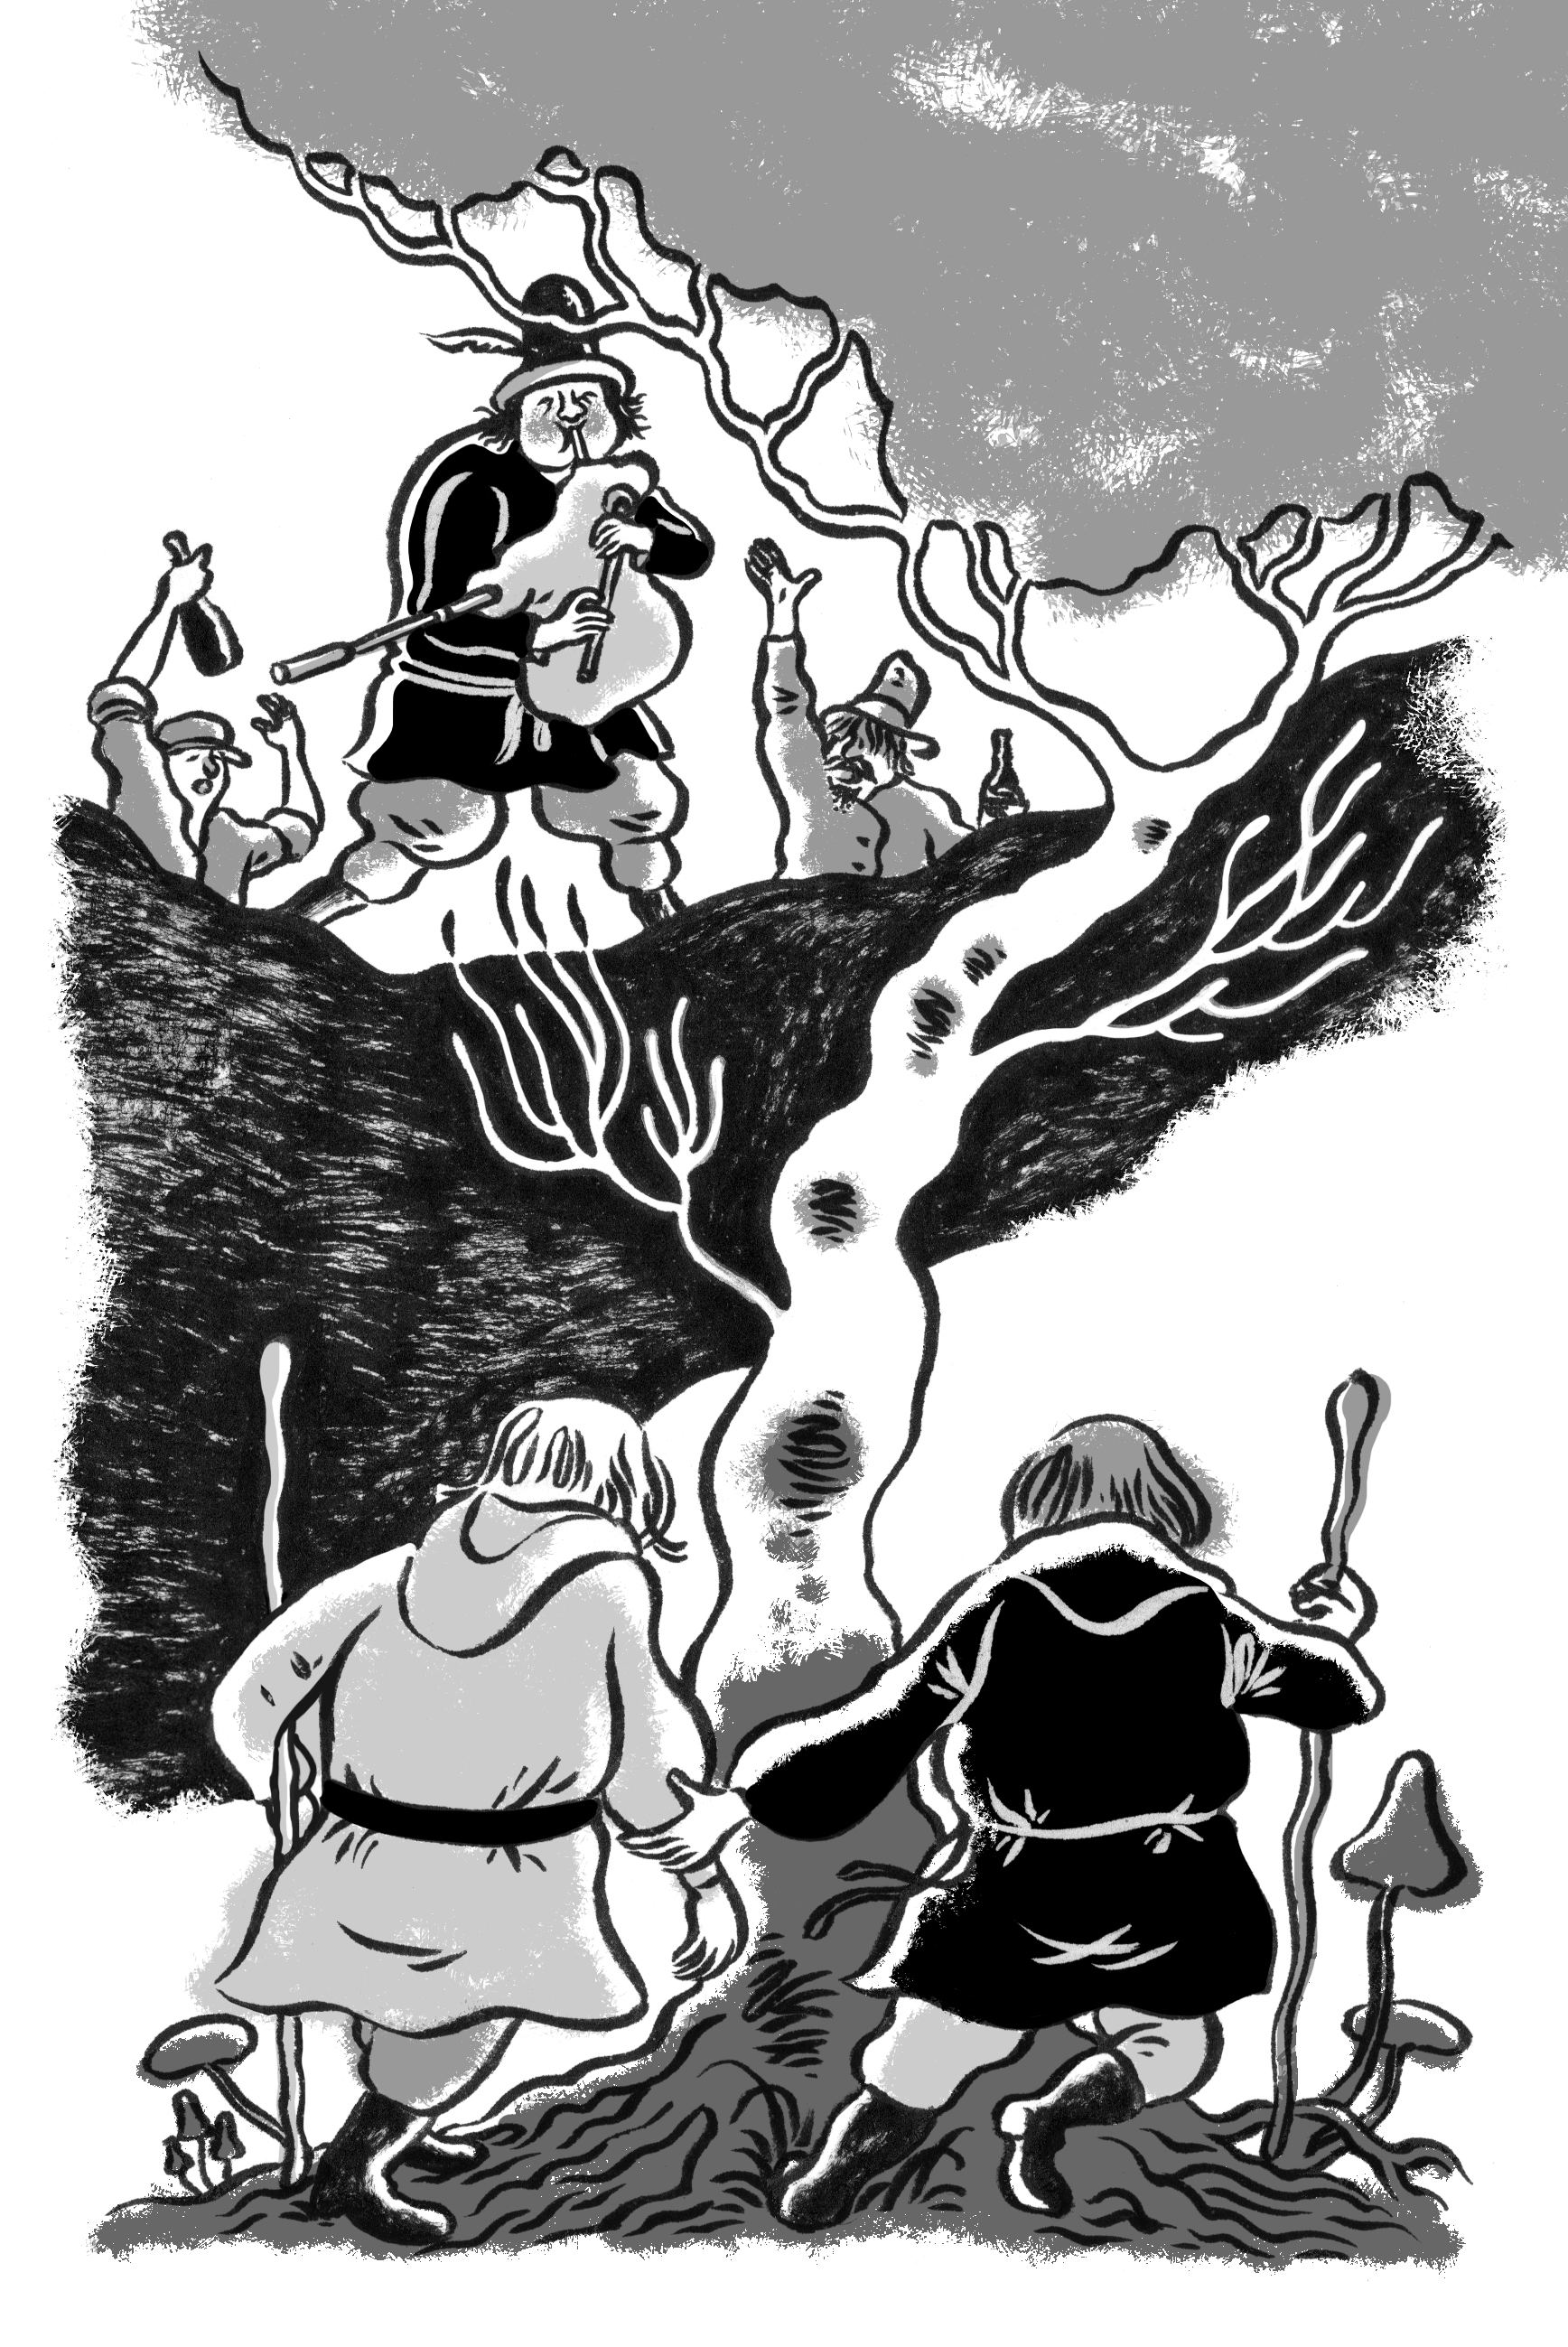
\includegraphics[width=\textwidth]{./images/PNLD0050-04.png}
\end{figure}

O enredo deste conto lembra alguma outra história? O filme \emph{O
Maravilhoso Mágico de Oz} (1939), baseado em livro de Frank Baum, tem
algo em comum com a parábola de Catarina? No \emph{Mágico de Oz}, a
menina Dorothy precisa seguir reto pela ``estrada de tijolos amarelos''
para encontrar o mágico de Oz, mas surgem distrações que a desviam do
caminho. Mesmo assim, Frank Baum (1856-1919) fazia parte de uma corrente
que afirmava que a função da literatura era divertir e entreter, e não
moralizar, papel que, segundo ele, caberia à família e à escola. Vale
estimular a discussão nesse sentido, dividindo a sala em dois grupos,
para que cada um defenda um ponto de vista.


\begin{enumerate}
\setcounter{enumi}{1}
\item ``Sobre como Kolka Pánkin viajou para o Brasil e sobre como
Pietka Erchóv não acreditou em nada'' (1928)
\end{enumerate}

\marginnote{\footnotesize\textbf{PARA VER}\\
\emph{O Mágico de Oz} (Victor Fleming, 1939)
}

Muito diversa do edificante conto de Catarina, a Grande, é a produção
de Daniil Kharms, fundador de um coletivo de vanguarda chamado \textsc{oberiu}
(1928) e precursor do teatro do absurdo na Rússia e hoje comparado a
autores como Franz Kafka e Eugène Ionesco. As obras de Kharms para
adultos só tiveram reconhecimento depois de 1990 (décadas depois de sua
morte trágica e precoce), mas os textos infantojuvenis dele, além de
virarem seu ganha"-pão, estavam entre os favoritos das crianças russas.
``O excêntrico Kharms, na década de 1920, vestia"-se com itens da
indumentária de Sherlock Holmes (seu herói favorito), participava
ativamente de círculos de vanguarda, praticava jiu"-jitsu, ioga e xadrez
e se interessava pelo ocultismo e pela cabala'' (\textsc{mountian}, 2021, p.
359). ua irreverência se reflete na imaginação solta suas obras, como
lemos neste conto.

\begin{figure}[ht!]
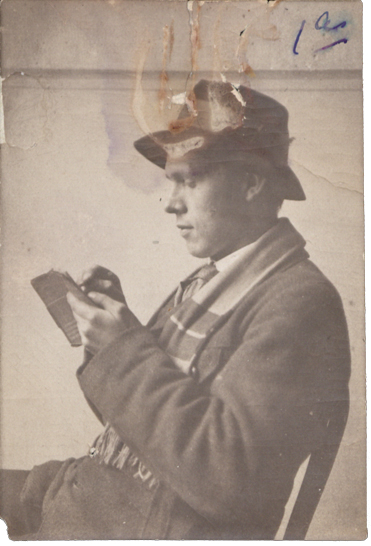
\includegraphics[width=\textwidth]{./images/PNLD0050-05.png}
\end{figure}

O que chama a atenção no modo como Kolka e Pietka lidam com fantasia e
realidade? Os dois materializam essa oposição em diálogos hilários, em
que um está sempre contradizendo o outro. A história desses dois meninos
de Petersburgo que fazem uma viagem imaginária ao Brasil tem um humor
que se constrói pelo ilógico, insólito e irracional: ``Pietka'', disse
Kolka, ``olhe só que Brasil!''. ``E isto aqui é o Brasil?'', perguntou
Pietka. ``Seu tonto, será que você mesmo não vê?'', disse Kolka. Aqui, o
professor pode introduzir brevemente a noção de \emph{nonsense}, à qual
voltaremos na pós"-leitura.

Questões sugeridas: A verossimilhança é importante para a história? A
lógica da realidade cotidiana se aplica ao enredo? Será que todo texto
deve conter um sentido lógico e racional? É possível definir as
fronteiras entre realidade e fantasia no conto?

O texto de Kharms trabalha com uma visão bem"-humorada e estereotipada
de Brasil que se disseminou na Rússia nos anos 1920. Pode ser que os
alunos já tenham ouvido falar em estereótipo, por isso valeria perguntar
se alguém poderia explicar o termo. Outras questões sugeridas: os
educandos conhecem algum estrangeiro, têm exemplos de estereótipos sobre
o Brasil que são repetidos em culturas estrangeiras? O que o estudante
acha que os russos pensam sobre o Brasil hoje? E o que ele conhece sobre
a Rússia? Os educandos podem pesquisar pela internet e apresentar alguns
estereótipos sobre a Rússia, fazendo uma verificação sobre a veracidade
deles e mostrá"-los à classe. Esta atividade poderá ser complementada com
uma proposta de escrita que sugerimos para a pós"-leitura.

\pagebreak

\subsection{Pós"-leitura \textsc{i}}

\marginnote{\footnotesize\textbf{PARA LER}\\
Sobre os estereótipos do Brasil na Rússia
(\emph{Estado de S. Paulo,} 04/10/19):\\
\url{https://bit.ly/3kYgnMv}
}


Espera"-se que os educandos assimilem as questões básicas que envolvem
a escrita de um conto: uma narrativa mais breve, com ênfase naquilo que
é essencial à história (com poucas personagens). À diferença da novela e
do romance, elimina as análises minuciosas e as complexidades do enredo,
delimitando o tempo e o espaço. No trabalho com contos, é importante que
os estudantes assimilem a maneira como o escritor recriou um evento real
ou criou um evento ficcional, que tipo de tratamento literário deu às
personagens e à narração (primeira ou terceira pessoa), e qual foi o
trabalho envolvido de seleção e de harmonização dos elementos
selecionados (por exemplo, normalmente o passado das personagens é
descrito em poucas linhas no conto, pois a narrativa fica concentrada em
um episódio particular).

O educador pode incentivar debates sobre alguma ideia contida no
texto, realizar atividades escritas e orais ou avaliações, com o
objetivo de aferir o desempenho dos alunos e alunas em relação à leitura
e compreensão dos contos.

Exercícios de escrita divertidos podem ser sugeridos na fase
pós"-leitura. Pode"-se, por exemplo, propor aos alunos que invertam a
locação do conto de Kharms, em uma redação de uma página: ``Sobre como
José Silva viajou para a Rússia e sobre como João Santos não acreditou
em nada'', ou uma variante feminina.

De quais histórias que usam do fantástico, do mundo imaginário e do
\emph{nonsense} o estudante se recorda? Talvez o filme \emph{Alice no
País das Maravilhas} (dir. Tim Burton, 2010), baseado no livro homônimo
de 1865 de Lewis Caroll? Este é considerado, junto com Edward Lear
(1812-1888), ``um dos pais da literatura \emph{nonsense} vitoriana''
(\textsc{lear}, 2016, p. 13) --- e ambos foram referência para Kharms. O termo
\emph{nonsense} (``sem sentido''), no contexto literário, foi tomado de
empréstimo do título de um livro de Lear: \emph{A book of nonsense}
(\emph{Um livro de nonsense}), de 1846. A temática da viagem a lugares
fantásticos é uma permanente na obra de Lear, que, com problemas
respiratórios, percorreu diversos países europeus em busca de
tratamento: ``Se os cenários `exóticos' inspiravam os desenhos de Lear,
também as pessoas, as línguas e os costumes diversos que encontrou
serviram"-lhe de inspiração''. (\textsc{lear}, 2016, p. 17) Outro que parece
seguir a linha do \emph{nonsense} de Lear é o brasileiro Sérgio
Capparelli (1947), cuja obra poética é pura viagem ao mundo mágico
infantojuvenil. Seu poema ``O Buraco do Tatu'', em que o bichinho
percorre o mundo apenas cavando túneis, pode ser lido ao lado do texto
de Kharms. Reparemos no seguinte trecho do poema:

\begin{verse}
O tatu cava um buraco\\
À procura de uma lebre,\\
Quando sai pra se coçar,\\
Já está em Porto Alegre.

O tatu cava um buraco\\
E fura a terra com gana,\\
Quando sai pra respirar,\\
Já está em Copacabana.

O tatu cava um buraco\\
E retira a terra aos montes,\\
Quando sai pra beber água,\\
Já está em Belo Horizonte.

(apud \textsc{kersley}, 2011, p. 337)

\end{verse}

\begin{figure}[ht!]
\includegraphics[width=\textwidth]{./images/PNLD0050-15.png}
\end{figure}

Após a leitura do restante do livro em casa, outros temas podem ser
trabalhados. Muitos protagonistas são púberes nos contos. Seria
interessante que se fizesse uma tipologia das personagens crianças e
adolescentes. Por exemplo, o menino acrobata, Serguei, que recupera o
cão em ``O poodle branco'', ou o garoto de ``Bobinho'', de Nikolai
Leskóv. Leskóv tinha uma religiosidade particular que se
manifesta neste conto: o ``bobinho'' tem uma alma generosa, é desapegado
de tudo e está sempre pronto a sofrer pelo próximo, e por isso é
considerado um tolo. O autor aqui descreve uma personagem com traços de
\emph{iuródivyi}, figura embrenhada na cultura popular russa, de caráter
religioso, definida como um misto de louco e profeta. Fazendo uma
pequena digressão, outro ponto a ser trabalhado na história de Leskóv é
o formal: o autor utiliza elementos dos contos populares russos, como a
oralidade e a narrativa da experiência (cujos aspectos podem ser
aprofundados pelo professor no texto de Walter Benjamin, \emph{O
narrador}, que mencionamos nas sugestões de leitura). No texto de
Leskóv, diferentemente de um texto informativo de jornal, os leitores se
tornam quase ouvintes. Enfim, depois de feita uma galeria de
personagens, o educando poderia apontar com qual ele mais se identifica
e por quê.

\marginnote{\footnotesize\textbf{PARA VER}\\
``Esqueci como se chama'', dir. Luis Felipe Labaki.
Encenação de conto de Daniil Kharms.\\
\url{https://www.youtube.com/watch?v=TynrL12SQ6U}
}

\paragraph{Tempo estimado} Quatro a cinco aulas de 50 minutos.

\subsection{Pós"-leitura \textsc{ii}}

\paragraph{Tema} \emph{Podcast} de audiocontos.

\BNCC{EM13LP16}
\BNCC{EM13LP17}
\BNCC{EM13LP18}
\BNCC{EM13LP28}
\BNCC{EM13LP29}
\BNCC{EM13LP34}
\BNCC{EM13LP45}
\BNCC{EM13LP46}
\BNCC{EM13LP52}
\BNCC{EM13LP53}
\BNCC{EM13LGG703}

\paragraph{Conteúdo}
Criação de um episódio de \emph{podcast} literário com análise de um dos
contos e leitura de trechos.

\marginnote{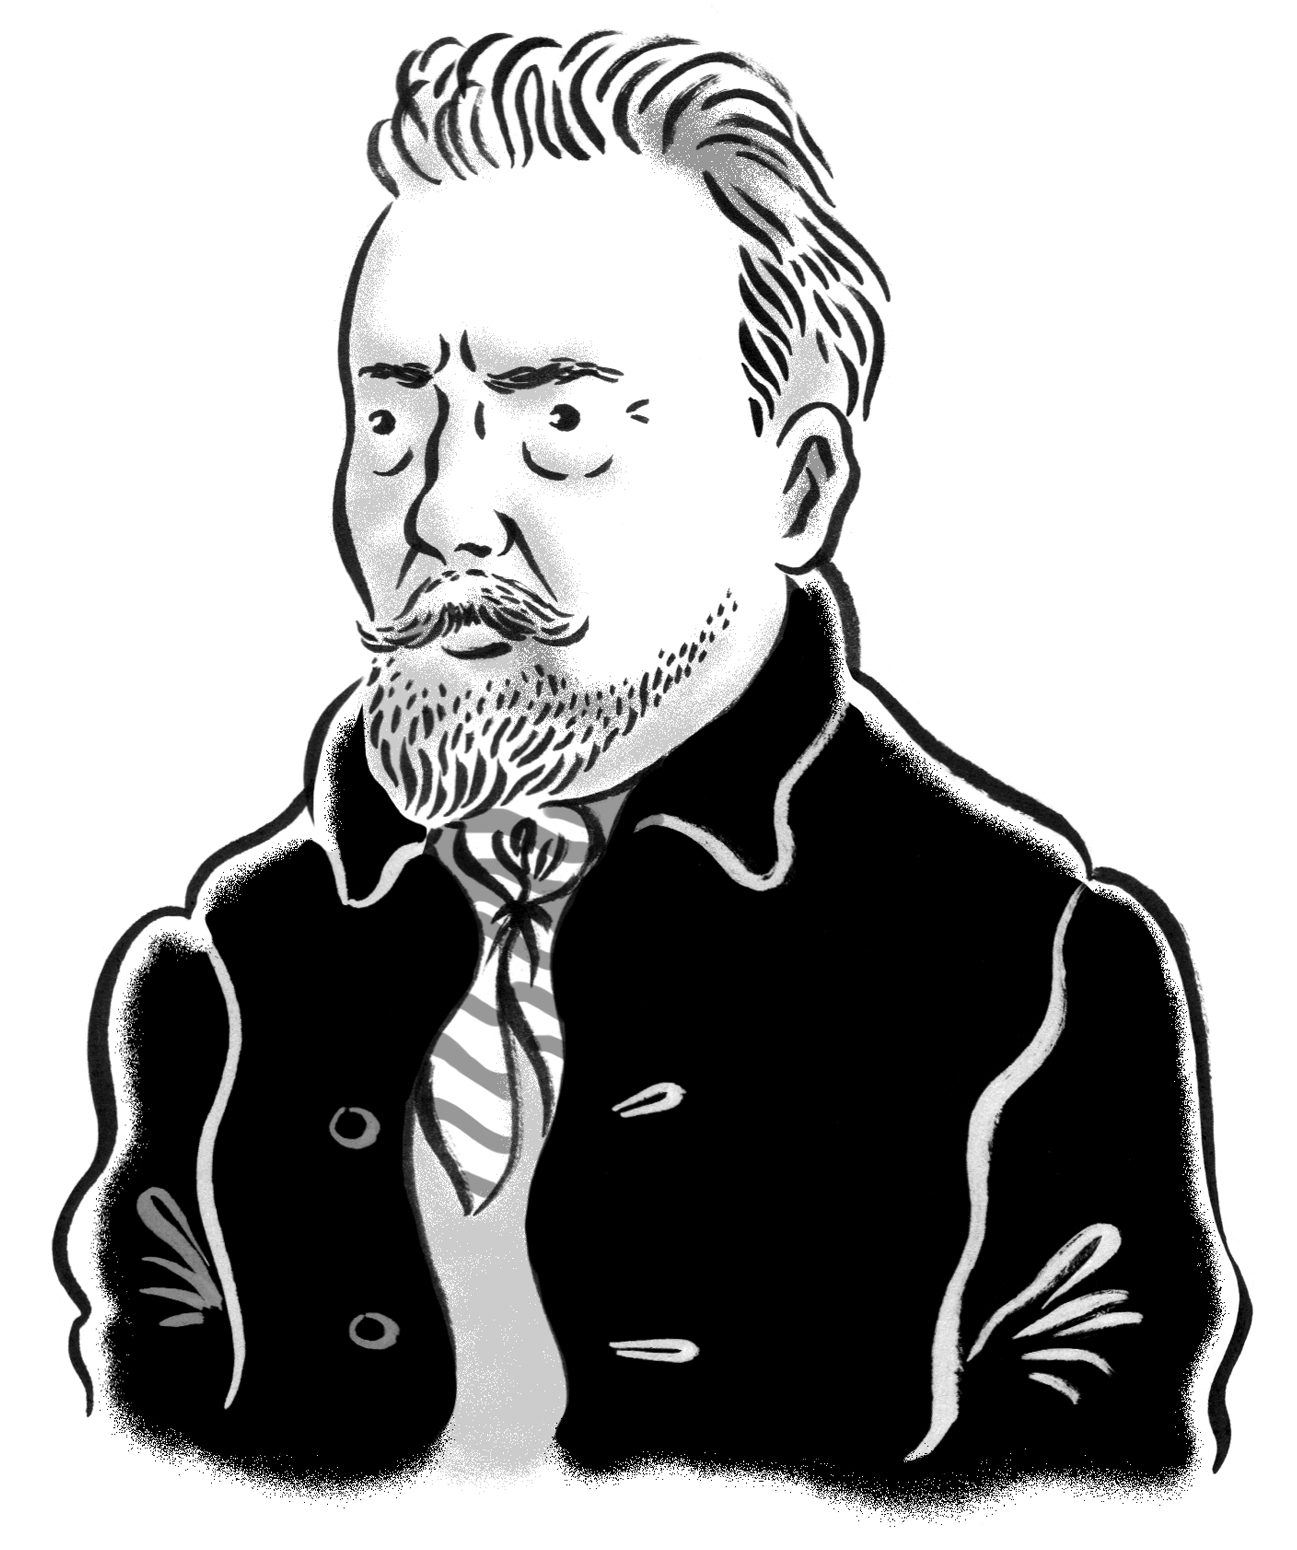
\includegraphics[width=5cm]{./images/PNLD0050-06.png}}

\paragraph{Objetivos}
Incentivar o jovem leitor a novos letramentos, multiletramentos e
multimodalidades por meio da produção cultural digital em grupo.

\paragraph{Justificativa}
A realização de um episódio de \emph{podcast} literário visa a
diversificar as produções culturais contemporâneas ao mesmo tempo que se
amplia o repertório de clássicos estrangeiros, possibilitando ao jovem
absorver a cultura impressa e ir além com a multimodalidade. A atividade
incentivará o letramento em novas mídias, permitindo que todos sejam
produtores, imbricando ainda mais as práticas de leitura e produção,
consumo e circulação de textos.

\paragraph{Metodologia}
A ideia é dividir a sala em grupos de três ou quatro alunos.
Inicialmente, após escolherem um ou dois contos a serem trabalhados,
fazem um fichamento do texto e, a partir disso, juntos, escrevem um
texto analítico, do qual sairá o roteiro do \emph{podcast} literário. O
episódio pode conter trechos lidos da obra, de modo a torná"-lo mais
interessante --- um recurso para enriquecer a leitura desses excertos é
a multiplicidade de locutores no caso de diálogos, além do narrador. A
gravação poderá ser feita pelo celular, editada por aplicativos simples
no aparelho e publicada em serviços como o \emph{Spotify} ou
\emph{SoundCloud}. Uma opção no caso de impossibilidade de acesso a
esses equipamentos é a leitura dramática dos contos em sala de aula.

\paragraph{Tempo estimado} Cinco a seis aulas de 50 minutos.


\subsection{Pós"-leitura \textsc{iii}}

\paragraph{Tema} Romantismo, realismo e outras estéticas literárias.

\BNCC{EM13LP52}

\paragraph{Conteúdo}
Características do romantismo, do realismo e de outras tendências
presentes nos \emph{Contos russos juvenis}.

\paragraph{Objetivos}
Conectar a leitura dos \emph{Contos russos} \emph{juvenis} ao currículo
escolar de literatura do ensino médio, auxiliando os alunos a
identificarem nos textos elementos dos períodos literários pertinentes.

\paragraph{Justificativa}
Esta proposta de letramento busca a via curricular do ensino médio ao
propor que o estudante aplique os conhecimentos literários obtidos em
sala nos textos trabalhados.

\paragraph{Metodologia}
Algumas questões podem ser debatidas em sala de aula:

\begin{enumerate}
\item Romantismo
\end{enumerate}

Como lemos no prefácio do livro (\textsc{mountian}, 2021), a literatura
infantil despertou a atenção dos escritores durante o romantismo, quando
histórias fantásticas se destacaram, com dois mundos distintos, o da
realidade e o da fantasia. Ou seja, o leitor sabe distinguir quando o
narrador trata de uma e de outra. Um dos contos mais emblemáticos desse
momento é ``A cidadezinha da tabaqueira'' (1834), de Vladímir Odóievski
(1802--1869), em que um menino entra dentro de uma caixinha de música
--- os objetos que ganham vida deixam transparecer traços da obra de E.
T. A. Hoffman (1776--1822). A linguagem do conto tem um tom terno e
infantil, com o uso de onomatopeias. Questões sugeridas: O aluno sabe
que recurso linguístico é esse? Pode dar exemplos na obra? Poderia
versar sobre a interação dos elementos da caixinha de música? Eles
existem coletivamente, ou seja, um depende do outro, e a caixinha só
funciona com cada um fazendo a sua parte (uma espécie de ``alegoria da
sociedade''):

\begin{quote}
--- Zás, zás, zás --- respondeu a rainha ---, que menino desmiolado, que
menino tonto! Olha para tudo e não vê nada! Se eu não tocasse no
cilindro, o cilindro não giraria; se o cilindro não girasse, não
engancharia nos martelinhos, os martelinhos não bateriam, os sininhos
não tocariam; se os sininhos não tocassem, não haveria música! Zás, zás,
zás!

(\textsc{mountian}, 2021, p. 58)
\end{quote}

Além da prosa fantástica, no romantismo surge o interesse pelo
folclore, que se refletiu no florescimento de estudos folclóricos
russos, como expressão de nacionalismo. Histórias populares,
transmitidas oralmente, passaram a ser coletadas e sistematizadas. Caso
mais representativo é o da coletânea \emph{Contos russos populares}
(1865-1863)\emph{,} de Aleksandr Afanássiev. São histórias
simbolicamente muito ricas e marcadas pela oralidade, sem trazer em
geral refinamento literário: quem começou a dar forma poética a elas foi
Aleksándr Púchkin (1799-1837), o poeta mais amado da Rússia. De criação
espontânea, elas fazem parte do que André Jolles chamou de ``formas
simples''. (\emph{apud} \textsc{gotlib}) Nossa coletânea não traz contos
populares russos em si, mas procedimentos narrativos deles são
utilizados por autores como Leskóv e Sologub. Questões sugeridas:
Conhece alguma história do folclore brasileiro? Você ouviu a história de
alguém ou leu num livro? Você se identifica com ela?

\marginnote{\footnotesize\textbf{PARA LER}\\ ``Aleksandr Nikoláievitch Afanássiev e o conto popular russo'': dissertação de mestrado (\textsc{usp}) de Flavia Moino.\\
\url{https://teses.usp.br/teses/disponiveis/8/8155/tde-12092008-170622/publico/DISSERTACAO\_FLAVIA\_CRISTINA\_MOINO\_CAROLINSKI.pdf}
}

\begin{enumerate}
\setcounter{enumi}{1}
\item Realismo
\end{enumerate}

Em geral, as grandes obras
do realismo russo, escritas por nomes como Ivan Turguêniev (1818--1883),
Fiódor Dostoiévski (1821--1881) e Lev Tolstói (1828--1910), tangenciam
questões sociais e humanitárias. E a mesma tendência se revela nos
contos infantis, que respondiam a anseios de um momento histórico
conturbado, já que as reformas institucionais do tsar Alexandre \textsc{ii} nos
anos 1860 tiveram reflexo em toda a sociedade. A literatura
infantojuvenil passou a ser alvo de interesse de escritores e críticos.
Muitos nesse período achavam que crianças não tinham que ser poupadas da
realidade e que deveriam ler textos para adultos desde o início da
adolescência, uma concepção de infância diferente da de hoje. Mas Lev
Tolstói, além de escrever livros emblemáticos como \emph{Anna Kariénina}
e \emph{Guerra e Paz}, dedicou boa parte de sua vida a projetos
educacionais, editoriais e literários voltados exclusivamente para os
pequenos russos. Escreveu vários textos dedicados ao público juvenil que
se tornaram clássicos do gênero, como ``О prisioneiro do
Cáucaso''\emph{,} incluído na coletânea, conto tão conhecido na Rússia
que foi adaptado duas vezes para o cinema. ``Com ritmo contagiante e
temas universais (traição, amizade, esperança, audácia, etc.), o
narrador de Tolstói, que adota o ponto de vista russo, mantém o colorido
local ao descrever os tártaros, sem cair na caricatura simplória, usando
da técnica contrastiva e de uma linguagem saborosa e ao mesmo tempo
simples, sem excessos.'' (\textsc{mountian}, 2021, p.19).

\begin{figure}[ht!]
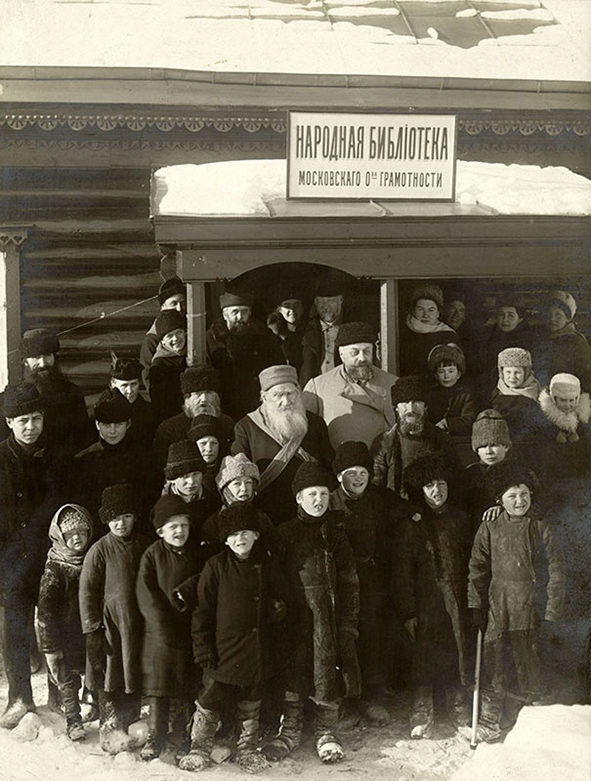
\includegraphics[width=\textwidth]{./images/PNLD0050-07.png}
\end{figure}

Embora suas obras tenham elementos românticos, Ivan Turguêniev (1818
--1883) é outro representante do realismo russo com textos que, sem
deixar de tocar em questões universais (como o amor e a morte), exploram
dilemas sociais. Os contos que integram suas \emph{Memórias de um
caçador} (1852), por exemplo, tiveram tanta repercussão na Rússia que
contribuíram para a emancipação dos servos (1861). Apesar de gostar de
crianças, o escritor quase não deixou obras para elas. No entanto, o
tristíssimo conto ``Mumu'' (1854), mesmo não tendo sido escrito
unicamente para o público juvenil, foi adotado pelas escolas russas e é
uma das histórias sobre animais mais conhecidas do país. ``Baseado numa
história real, retrata o duro destino da doce Mumu, a \emph{spaniel} de
Guerássim, um brutamontes surdo"-mudo, de caráter duro, mas inocente, que
todos temiam e de algum modo respeitavam.'' (\textsc{mountian}, 2021, p. 19).

\begin{figure}[ht!]
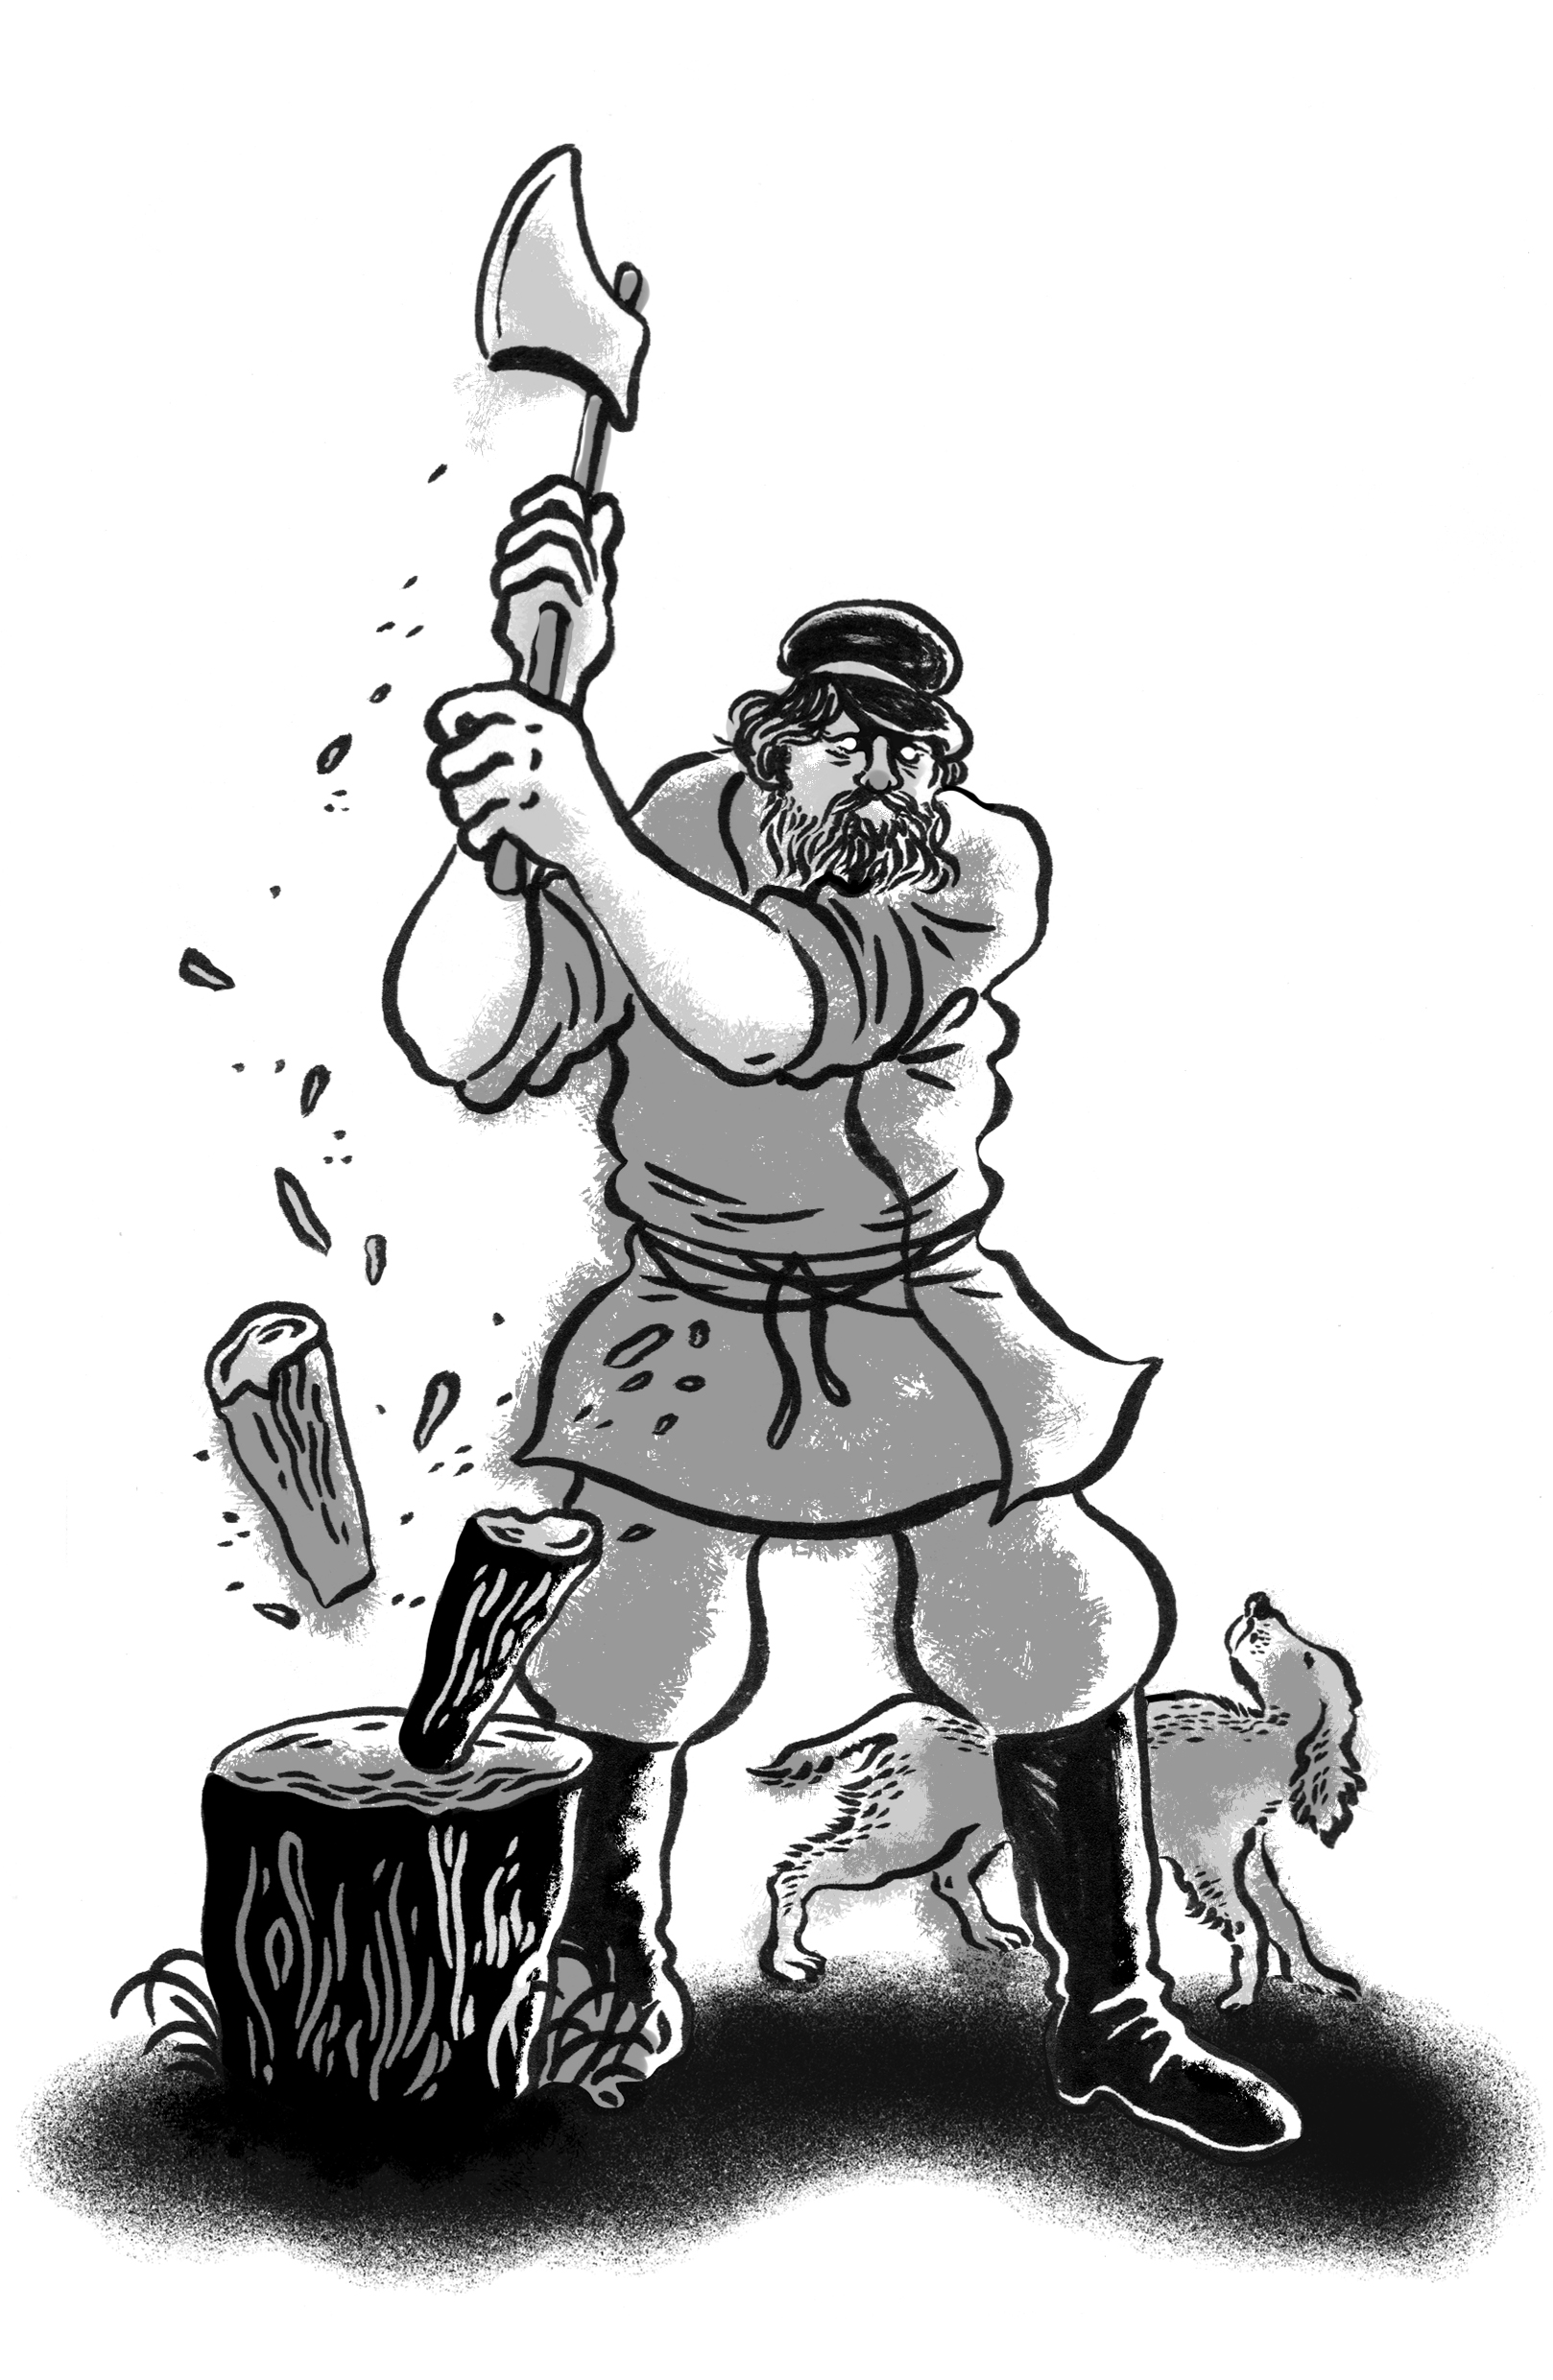
\includegraphics[width=\textwidth]{./images/PNLD0050-08.png}
\end{figure}

\begin{enumerate}
\setcounter{enumi}{2}
\item Novo realismo
\end{enumerate}

Contista por excelência e criador de um novo tipo de realismo, Anton
Tchékhov surge em dois textos da coletânea: ``Vanka'' (1896) e ``O
fugitivo'' (1887), ambos muito conhecidos na Rússia. No comovente
``Vanka''\emph{,} um menino órfão, vivendo em condições miseráveis,
``escreve uma carta ao seu avô para que venha buscá"-lo, uma carta sem
endereço que nunca chegará\ldots{}''. (\textsc{mountian}, 2021, p.361) Os contos
tchekhovianos mudaram o rumo da prosa curta mundial, construídos com
tanta sutileza que o leitor muitas vezes precisa de tempo para
enxergá"-la. Nádia Gotlib nota que neles a unidade tradicional, com
início, meio e fim, é rompida. Como lembra Boris Schnaiderman
(\emph{apud} \textsc{gotlib}, 2006, p. 27) em seu artigo ``Por falar em conto'':
``É justamente pelo meio que os seus contos inovam''; muitas vezes o fim
é inconclusivo neles; o que realmente ``importa está em detalhes quase
imperceptíveis ou no que foi deixado de dizer'' (\textsc{mountian}, 2021, p.21);
os enredos não têm um caráter grandioso e se voltam para episódios
cotidianos e aparentemente desimportantes. Além disso, Gotlib (2006, p.
25) observa que: ``A intenção de Tchékhov"-escritor realista é
repetidamente anunciada por ele mesmo: representar a verdade, que é `a
absoluta liberdade do homem, liberdade da opressão, dos preconceitos,
ignorância, paixões, etc.' E denunciar uma situação condenável''.

\begin{figure}[ht!]
\includegraphics[width=\textwidth]{./images/PNLD0050-03.png}
\end{figure}

Esse caráter de denúncia também define obras de Aleksándr Kuprin
(1870-1938) e de Lídia Avílova (1864-1943). Avílova tem o nome
geralmente ligado ao de Anton Tchékhov por ter escrito uma biografia do
autor e ter tido uma relação próxima com ele --- Tchékhov inclusive dava
conselhos sobre os textos dela, elogiados por Tolstói. Além disso,
aproximam"-na dele a temática social, a predileção pelo conto e algumas
marcas de estilo. Em ``Primeira mágoa'' (1912), temos a história
de Gricha, um jovenzinho que se vê diante de seu primeiro dilema ético.
Um dia, Ignát, o bom cocheiro a quem o menino havia se afeiçoado, foi
preso por ter fugido, antes de trabalhar na família de Gricha, com os
cavalos do antigo patrão, que tratava seu empregado como escravo.
Algumas questões podem ser colocadas aos educandos: O cocheiro deveria
ser preso? Qual foi a grande mágoa do menino? O que ele esperava do pai?


\begin{enumerate}
\setcounter{enumi}{3}
\item Simbolismo e outras tendências do início do século \textsc{xx}
\end{enumerate}

\marginnote{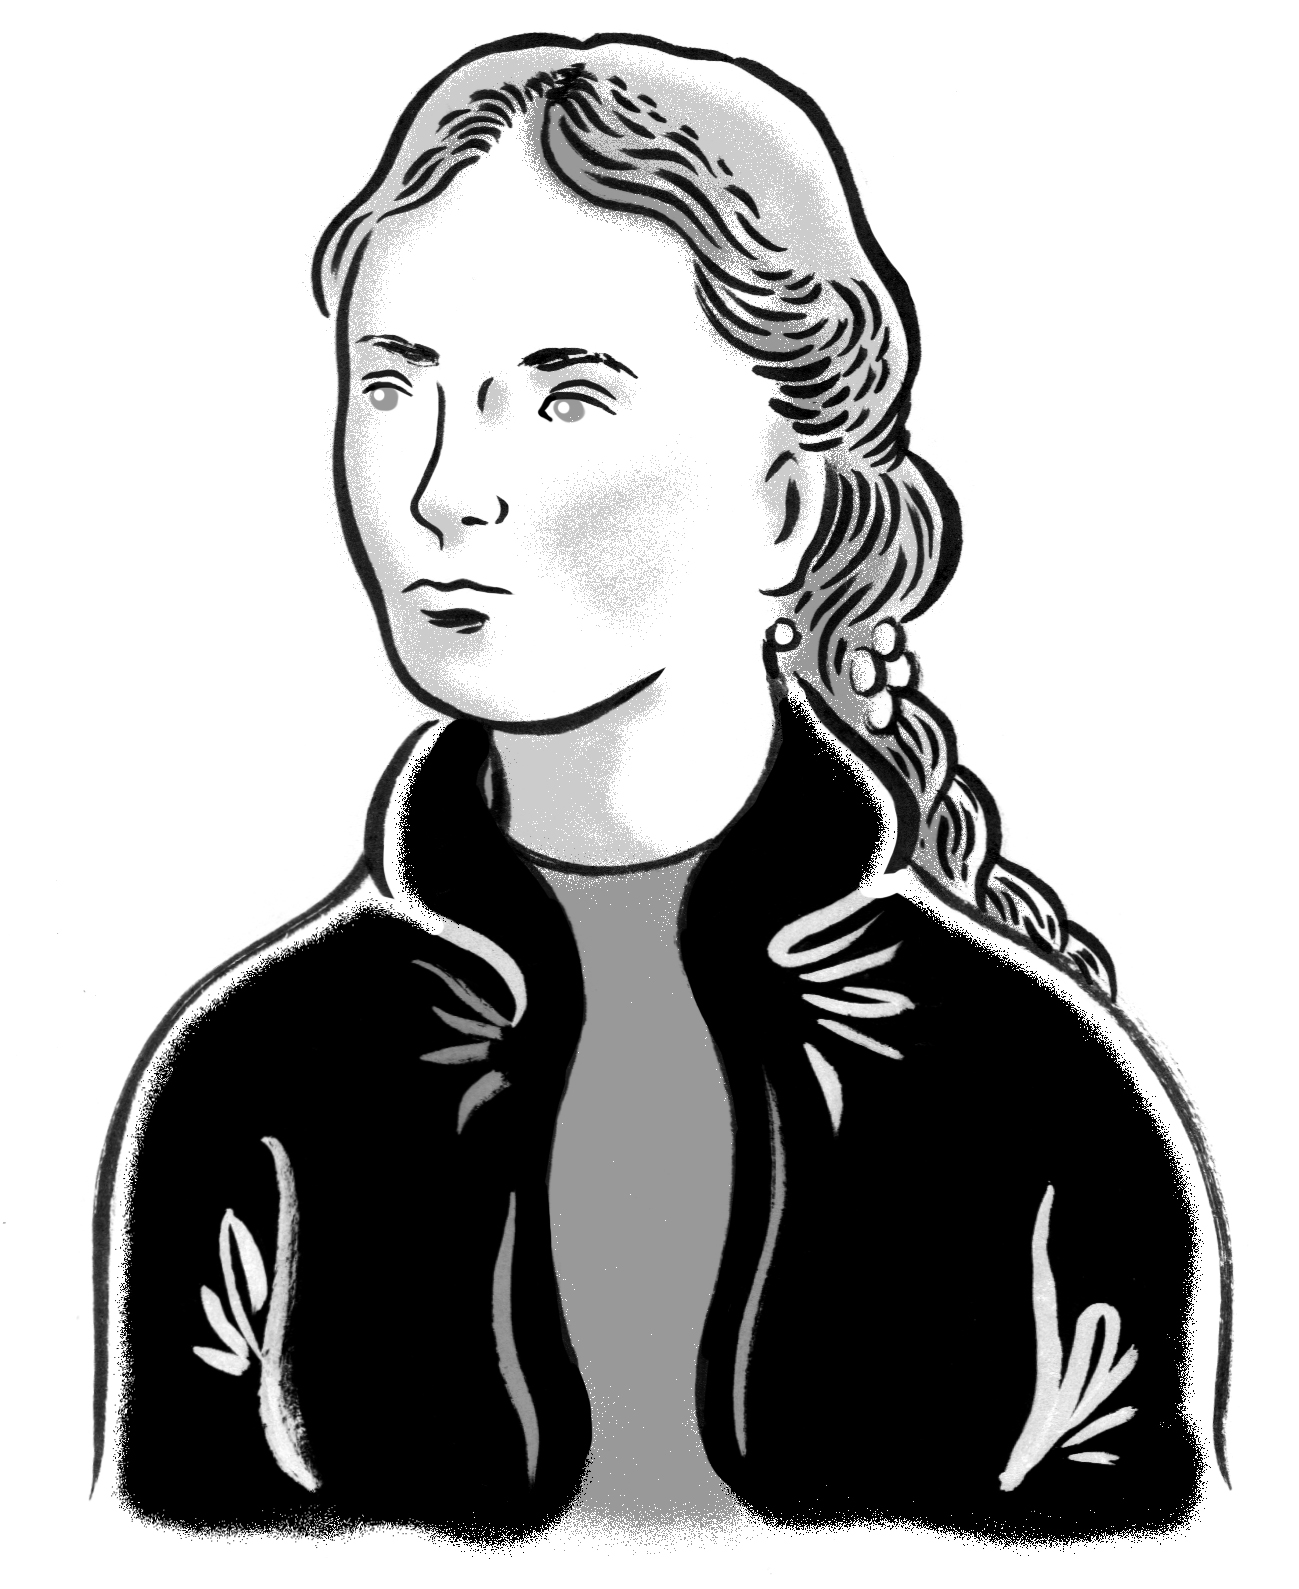
\includegraphics[width=5cm]{./images/PNLD0050-09.png}}

A Era de Prata, como se convencionou chamar a fase que vai do
simbolismo às diversas correntes de vanguarda, se estendeu por um
período curto da história russa, por cerca de trinta anos, mas deixou
criações impressionantes. O princípio dessa concentração de artistas
inovadores se deu no simbolismo russo, que teve seu ápice no começo do
século \textsc{xx}. Com o interesse simbolista pelo mito e pelo folclore, muitos
representantes desse movimento revisitaram o conto maravilhoso, como
Fiódor Sologub, que surge na coletânea com ``A filha do fabricante de
caixões'', história que traz uma mistura de mundos (típica do
escritor) e o tema da morte concentrados na protagonista, com um clima
sinistro e gótico que por vezes lembra as aparições de Catherine em
\emph{O Morro dos Ventos Uivantes} (1847), de Emily Brontë.

Prenunciando a nova literatura russa infantil, como destaca Mountian
(2021), está ``A pedrinha vermelha'', de Sacha Tchórny (1875-1937), que
ficou conhecido por seus textos satíricos. O conto foi escrito ao gosto
infantil, preservando o olhar da criança, e tem uma linguagem saborosa
com aliterações, criando onomatopeias que imitam a voz dos animais, já
que o protagonista escutava a conversa deles. O conto de Tchórny, pelo
caráter fantástico e até pelas onomatopeias, dialoga com ``A cidadezinha
na tabaqueira'', de Vladímir Odóievski (1803-1869).

\begin{figure}[ht!]
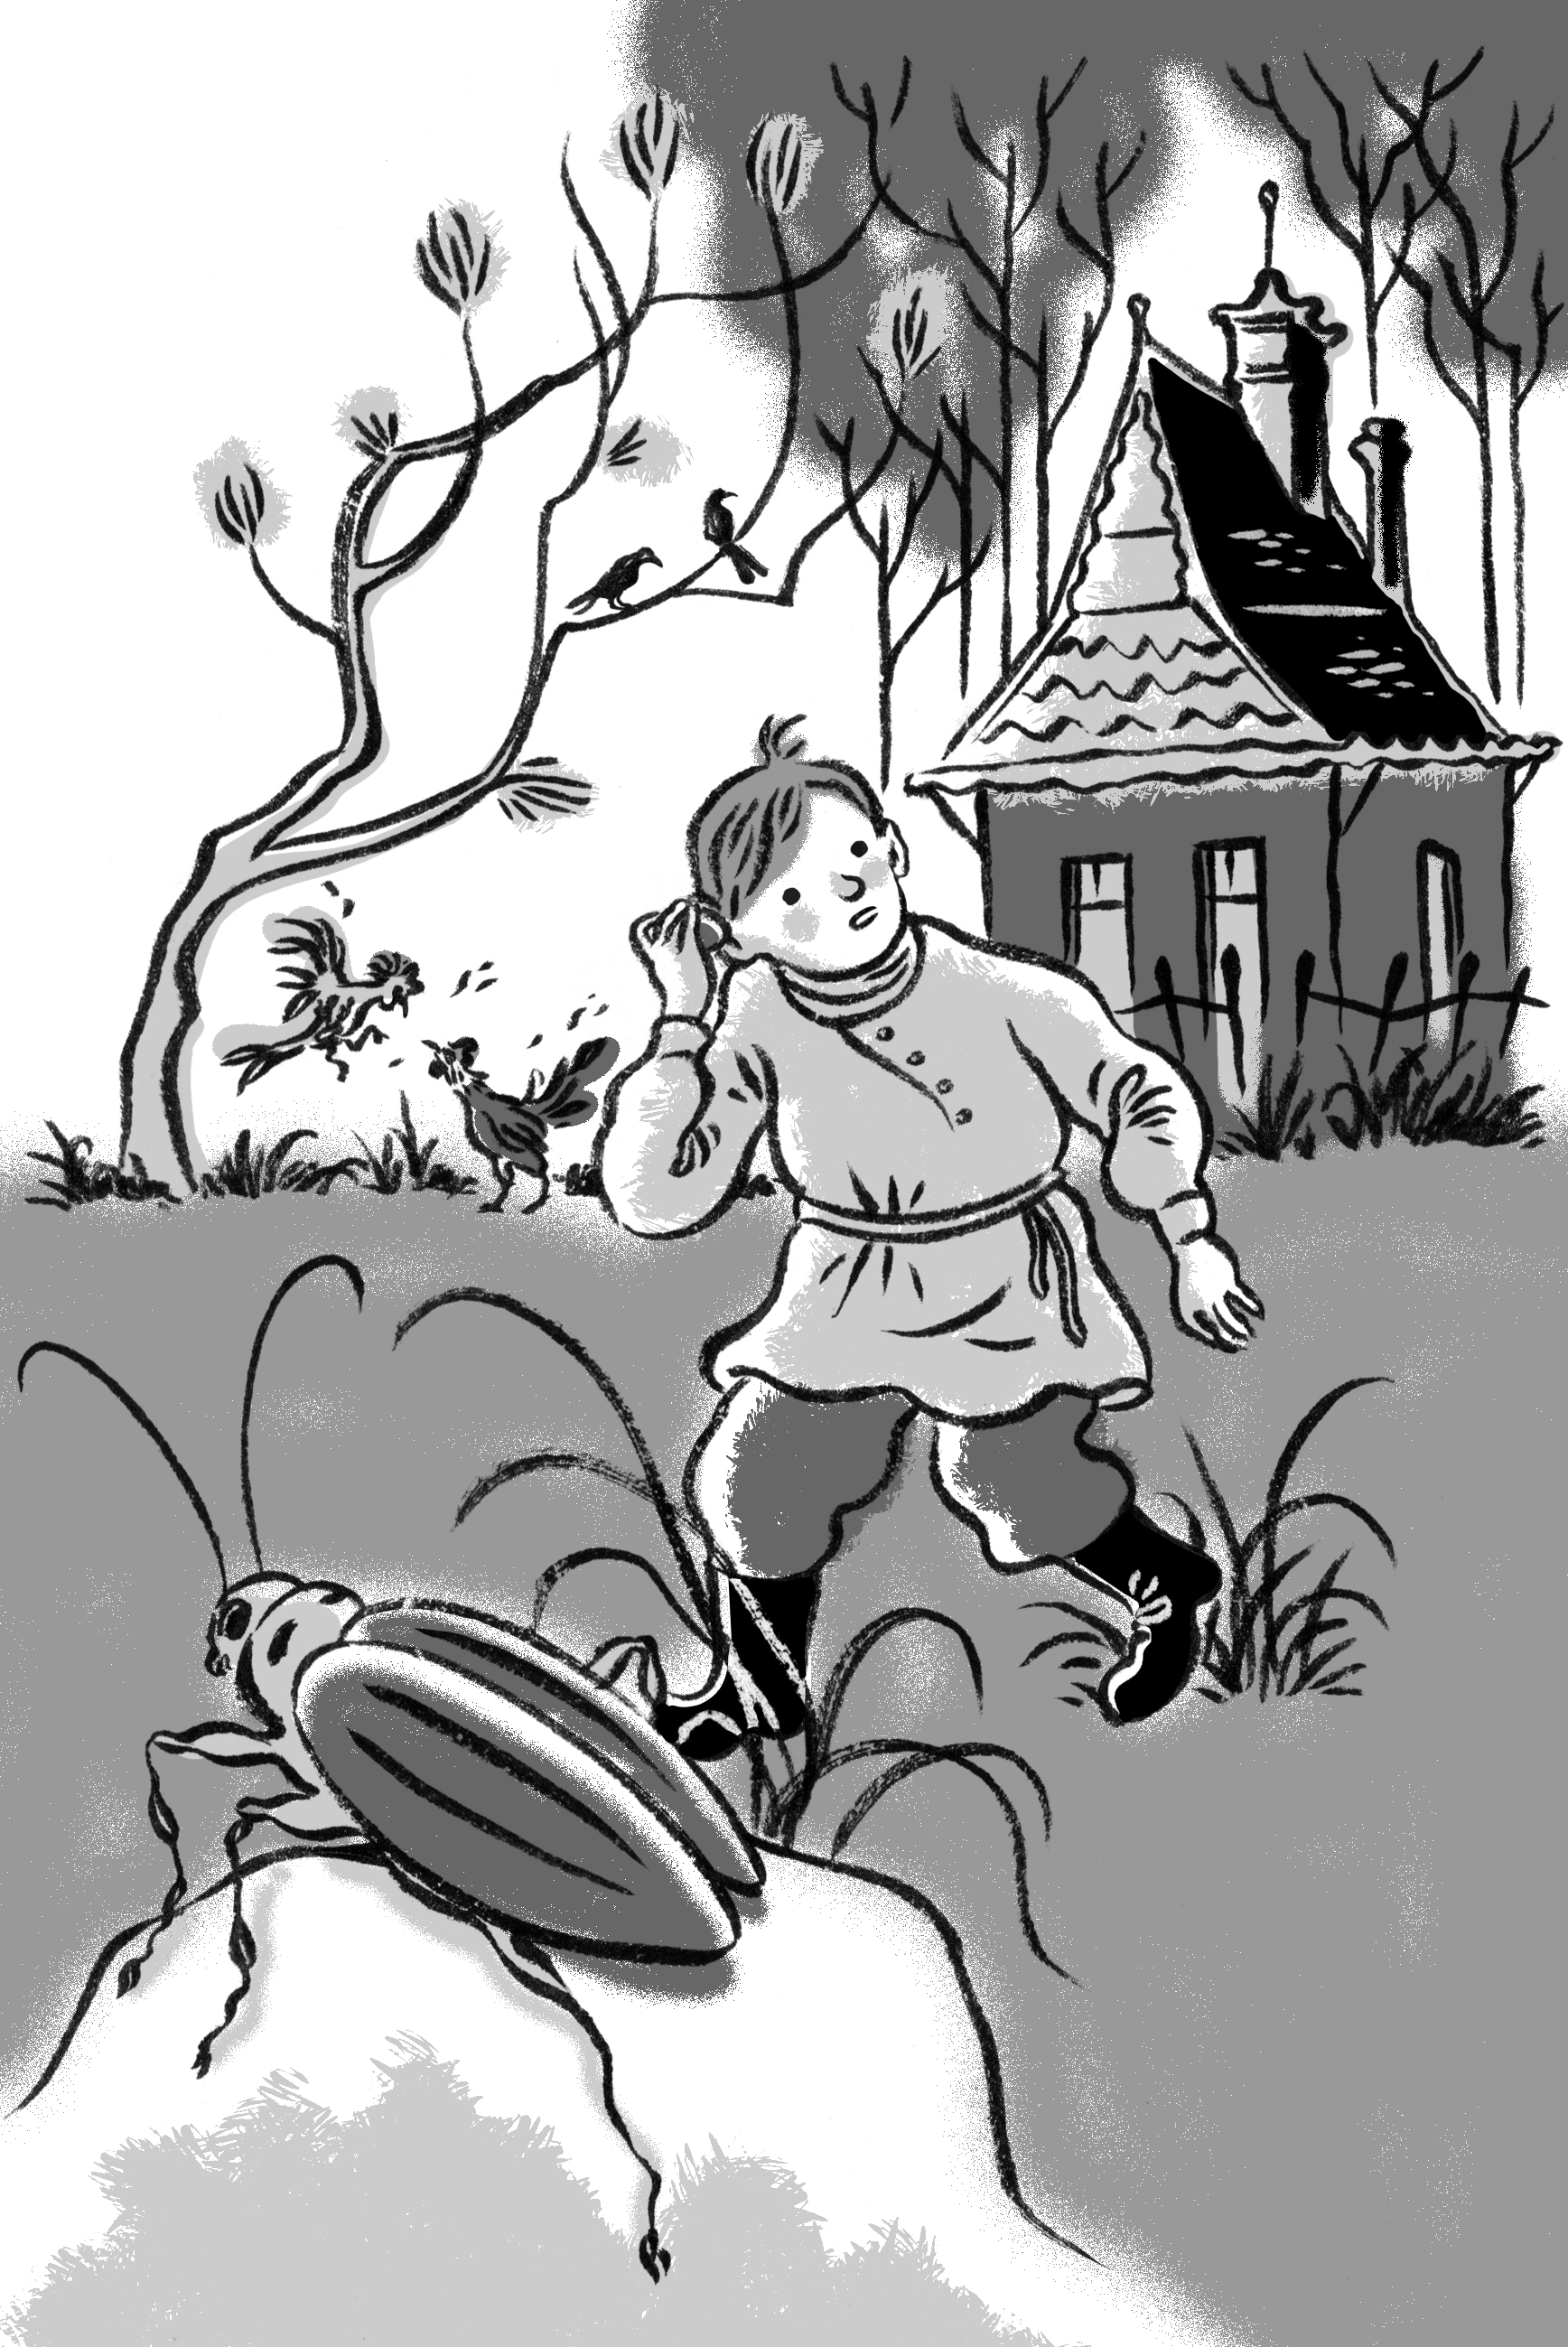
\includegraphics[width=\textwidth]{./images/PNLD0050-10.png}
\end{figure}

Questões sugeridas: O que é aliteração? O estudante pode dar algum
exemplo desse recurso linguístico? Os contos ``A pedrinha vermelha'' e
``A cidadezinha na tabaqueira'' têm pontos em comum? Como a realidade e
a fantasia se relacionam neles? São mundos distintos ou se misturam?

No início do séc. \textsc{xx}, a escritora predileta das moças russas era Lídia
Tchárskaia (1875--1937), que passava ao largo dos círculos artísticos.
``Tchárskaia produzia febrilmente e, por anos, tudo o que publicava
virava \emph{best"-seller}. Muitas de suas heroínas românticas,
sentimentais e positivas, de caráter marcante (não raro órfãs), movidas
por valores de moral elevada (bondade, amizade, generosidade), eram
popularíssimas na Rússia'', embora em geral não tenham conquistado o
respeito dos críticos (\textsc{mountian}, 2021, p.26) Tchárskaia enveredou por
vários gêneros e estilos e escrevia sem parar, mas, com a instauração do
regime soviético, as coisas mudaram. De autora preferida das russinhas,
ela tornou"-se uma figura indesejada --- teve seus livros proibidos nos
anos 1920, após uma enxurrada de críticas negativas dizendo, em geral,
que sua obra não condizia com os ditames do novo governo. A escritora
viveu na miséria, sem exercer a profissão, entre 1924 e 1938, quando
morreu.

Nos contos aqui apresentados, temos protagonistas femininas em vidas
cotidianas. Em ``A mãe\emph{'',} é retratado o duro ramerrão de uma
pobre viúva e, no fim, como ocorre no conto de Avílova, o filho Volódia
(Vladímir) passa por um processo de conscientização. Em ``A prova'', são
descritas as aflições de Nata na véspera de um exame que certamente
muitos estudantes vão reconhecer. Os alunos podem discorrer sobre o
narrador, o tempo usado (passado próximo ou longínquo, presente), sobre
a temática (cotidiana ou não).

\marginnote{\footnotesize\textbf{PARA VER}\\
``Prisioneiro das montanhas'', versão contemporânea
do conto de Tolstói (1996, Serguei Bodróv, \textsc{rus}, \textsc{caz})}

\paragraph{Tempo estimado} Quatro a seis aulas de 50 minutos.

\subsection{Pós"-leitura \textsc{iv}}

\paragraph{Tema} Oficina e sarau de minicontos.

\BNCC{EM13LP20}
\BNCC{EM13LP47}
\BNCC{EM13LP53}
\BNCC{EM13LP54}

\paragraph{Conteúdo}
Oficina para produção de minicontos autorais e sarau para apresentação.

\paragraph{Objetivos}
Incentivar a escrita e socialização da produção textual por meio dos
conhecimentos obtidos sobre o conto, promovendo um trabalho
protagonizado por estudantes do ensino médio.

\paragraph{Justificativa}
A partir da criação de uma atividade que promova articulação entre áreas
do conhecimento, a oficina favorecerá a autonomia dos alunos, além da
prática sistemática de leitura, pesquisa e escrita de textos com o conto
como base.

\paragraph{Metodologia}
Pode existir inspiração em um simples objeto inanimado? Segundo o mestre
contador de histórias colombiano Gabriel García Márquez, sim:

\begin{quote}
A coisa mais importante deste mundo é o processo de criação. Que tipo de
mistério é esse, que faz com que o simples desejo de contar histórias se
transforme numa paixão, e que um ser humano seja capaz de morrer por
essa paixão, morrer de fome, de frio ou do que for, desde que seja capaz
de fazer uma coisa que não pode ser vista nem tocada, e que afinal,
pensando bem, não serve para nada? Algumas vezes acreditei --- ou
melhor, tive a ilusão de estar acreditando --- que ia descobrir, de
repente, o mistério da criação, o momento exato em que uma história
surge.

{[}\ldots{}{]}

Dia desses, folheando uma revista \emph{Life}, encontrei uma fotografia
enorme. É uma foto do enterro de Hiroíto. Nela, aparece a nova
imperatriz, a esposa de Akihito. Está chovendo. Ao fundo, fora de foco,
aparecem os guardas com suas capas brancas, e mais ao fundo ainda, a
multidão com guarda"-chuvas, jornais e pedaços de pano na cabeça; e no
centro da foto, totalmente vestida de negro, aparece a imperatriz, num
segundo plano, solitária e muito magra. Vi essa foto maravilhosa e a
primeira coisa que me veio ao coração foi que ali havia uma história.
Uma história que, claro, não é a da morte do imperador, a que a
fotografia está contando, mas outra: uma história de meia hora. Fiquei
com essa ideia na cabeça, e ela continuou lá, dando voltas. Já eliminei
o fundo, me desfiz completamente dos guardas vestidos de branco, das
pessoas\ldots{} Por um momento, fiquei unicamente com a imagem da imperatriz
debaixo da chuva, mas logo descartei também. E então, a única coisa que
me ficou foi o guarda"-chuva. Estou absolutamente convencido de que
existe uma história nesse guarda"-chuva. (\textsc{márquez}, 2004 p.14-15)
\end{quote}

A ideia aqui é que o jovem escritor dê asas à imaginação e crie um conto
de duas a três páginas sobre um acontecimento real ou fictício,
aplicando os conceitos aprendidos em sala sobre o gênero. A oficina pode
se iniciar com uma troca de impressões sobre a coletânea e sobre a
futura redação, a qual os alunos devem trabalhar individualmente: ``No
fim, só uma pessoa escreve a história (\ldots{}) Porque é claro que as linhas
gerais da história podem ser elaboradas coletivamente, mas na hora de
escrever o roteiro, a tarefa tem de ser de um só''. (\textsc{márquez}, 1995,
p.13)

\paragraph{Tempo estimado} Três a quatro aulas de 50 minutos.

\section{Atividades 2}

Orientações gerais para a utilização dos temas e conteúdos
presentes na obra com uma abordagem interdisciplinar.

\paragraph{Tema} Cineclube Catarina: o contexto histórico do
surgimento de uma literatura infantojuvenil russa.

\BNCC{EM13LP01}
\BNCC{EM13LP02}
\BNCC{EM13CHS203}
\BNCC{EM13CHS603}

\paragraph{Conteúdo}
O tempo"-espaço em que começou a florescer a literatura infantojuvenil na
Rússia, ou seja, em meio ao ápice do chamado ``despotismo esclarecido''
russo: o reinado de Catarina \textsc{ii} (Catarina, a Grande).

\paragraph{Objetivos}
Situar o jovem leitor no contexto histórico russo e mundial em que se
inseriu o reinado de Catarina \textsc{ii}, que ajudou a dar os primeiros passos
para a consolidação da literatura infantojuvenil russa.

\paragraph{Justificativa}
A literatura infantojuvenil passou a ser valorizada na Rússia no
romantismo, a partir da segunda década do século \textsc{xix}. Mas, ainda no
final do século anterior, houve eventos importantes para a consolidação
das letras russas infantis (como a criação da revista \emph{Leitura
infantil para o coração e a razão}) e um aumento de publicações voltadas
para esse público. (\textsc{mountian}, 2021, p. 12) Além disso, foi no fim do
século \textsc{xviii} que surgiu este que é considerado o La Fontaine russo: Ivan
Krylóv (1769--1844). A própria imperatriz Catarina, a Grande (que reinou
de 1762 a 1796), pregando os ideais de Rousseau, achava que conhecimento
do mundo deveria ser adquirido desde a infância pela leitura. Prussiana
de nascimento, ela manteve permanente correspondência com filósofos
franceses, como Voltaire, que chegou a visitar a corte de São
Petersburgo, então capital russa. As ``Luzes'' da imperatriz foram, porém,
mais lenda que realidade em alguns âmbitos: embora ela tenha realizado
reformas administrativas importantes, incentivando as universidades de
Moscou e São Petersburgo, estimulando as ciências naturais, apoiando a
agricultura na Ucrânia e nas margens do Volga, foi implacável com
antagonistas políticos e, durante seu reinado, foi criada a Zona de
Assentamento para Judeus, que restringia a circulação deles no restante
do império.

\marginnote{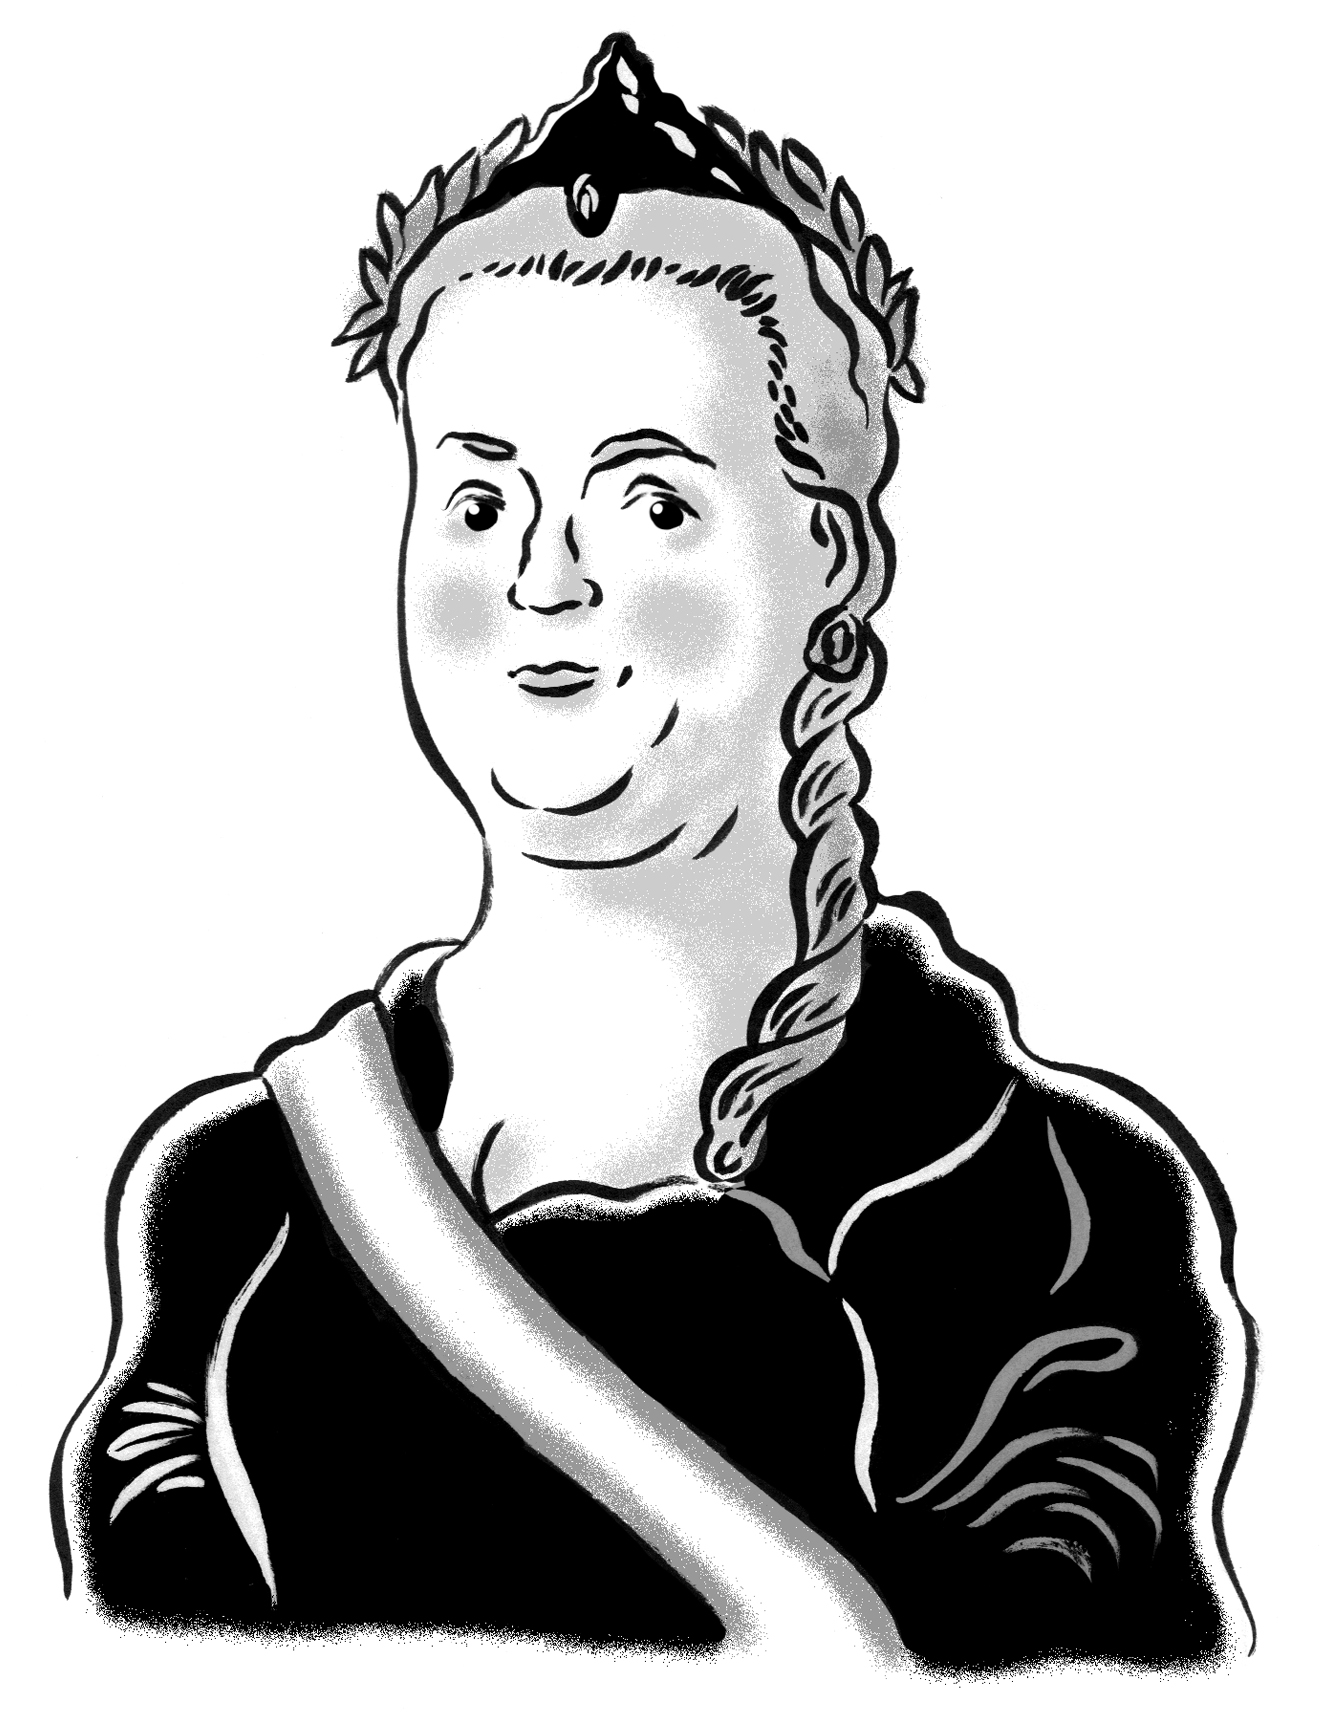
\includegraphics[width=5cm]{./images/PNLD0050-11.png}}

\paragraph{Metodologia}
Após a expansão do Grão"-Ducado de Moscou para leste (Urais e Sibéria),
noroeste e sul, a Rússia se tornou um dos reinos que passou por reformas
inspiradas no Iluminismo. Foi no reinado do tsar Pedro, o Grande, que o
país começou a adotar costumes da Europa ocidental, com imposições que
iam desde a obrigatoriedade de todo nobre se barbear e usar trajes
europeus (os nobres russos usavam barbas longas e vestimentas à moda
oriental) e de aprender a ler e a escrever, até a impressão do primeiro
jornal russo, o \emph{Notícias} (\emph{Viédomosti}), em janeiro de 1703.
Tudo isso após o jovem Pedro ter realizado uma inspiradora jornada de
dois anos por países europeus que começara em 1697. Alguns anos depois
de retornar, o tsar determinou a construção de São Petersburgo (capital
do império a partir de 1712) e passou a introduzir costumes europeus na
Rússia, ignorando as queixas dos nobres.


Mas a época áurea do chamado ``despotismo esclarecido'' ocorreu no reinado
de Catarina, a Grande (1729--1796), ``cuja correspondência com Voltaire
tornou"-se célebre''. Ela também escreveu uma cartilha para os netos em
1781 e alguns textos e diálogos edificantes. Duas obras suas são
consideradas pioneiras da prosa infantil russa: ``Conto do Tsarévitche
Cloro'' (1781) e ``Conto dо Tsarévitche Fеvei'' (1783),
que, ``sem viés nacionalista'', ressaltam valores universais, como
justiça e bondade, como observado no prefácio. (\textsc{mountian}, 2021, p.11)

Para realizar esta atividade, sugerimos que os alunos pesquisem,
individualmente ou em grupo, pela internet ou na biblioteca, sobre o
reinado de Catarina, a Grande, e sobre o contexto mundial que permitiu o
desenrolar do chamado ``despotismo esclarecido''.

\marginnote{\footnotesize\textbf{PARA LER}\\ ``De calendários a batatas: 5 legados de Pedro, o Grande, para a Rússia'' (\emph{Russian Beyond,} 23/09/17).\\
\url{https://bit.ly/2OxXrYX}
}

Em seguida, podem ser exibidos trechos da série \emph{Catarina, a
Grande} (Philip Martin, 2019, disponível no \textsc{hbo go}), principalmente do
primeiro capítulo, que vale ser mostrado integralmente. Após a exibição,
a sala formará uma roda de conversa para debater alguns pontos: Quais
tendências iluministas de Catarina são retratadas pelos autores na
série? O aluno pode fazer menções à relação da soberana com Voltaire e
às concepções dela sobre casamento e divórcio retratadas no episódio; à
sua ideia de abolir a servidão (o que só será realizado, efetivamente,
pelo tsar Alexandre \textsc{ii} em 1861); à presença de Thomas Dimsdale (médico
inglês que desenvolveu um método de prevenção de varíola por inoculação
para proteção de cepas mais virulentas e foi convidado para ir ao
Império Russo em 1768 por Catarina, para inocular a imperatriz, o filho
e 140 membros da corte --- realizando a ``variolação'' antes do ``pai da
imunologia'' Edward Jenner, que testou seu procedimento de vacinação
contra a varíola em 1796); à escrita, em seu quarto, sobre ideias de
igualdade diante da lei. Na via contrária, quais indícios de despotismo
poderiam ser apontados? Quem foi Ivan \textsc{vi}, o ``prisioneiro número 1'' de
Shlisselburg? E por que a relação de Catarina com o filho, Paulo, era
tão turbulenta? Como a política externa russa de Catarina \textsc{ii} deu
continuidade à de Pedro I? Após se aprofundar mais na história da
imperatriz russa, o estudante consegue captar outras nuances na obra
escrita para o neto que aparece em \emph{Contos russos juvenis}?

\paragraph{Tempo estimado} Três a quatro aulas de 50 minutos.

\subsection{Pré"-leitura}

\paragraph{Tema} A mulher nos \emph{Contos russos juvenis}.

\BNCC{EM13LP01}
\BNCC{EM13LP46}
\BNCC{EM13CHS101}
\BNCC{EM13CHS102}
\BNCC{EM13CHS201}
\BNCC{EM13CHS603}

\paragraph{Conteúdo}
Análise da figura feminina, sobretudo a da mãe, na literatura russa ao
longo de um período que cobre desde o século \textsc{xviii} ao início do \textsc{xx}.

\paragraph{Objetivo}
Abranger uma diversidade de temas e de contextos sociais, culturais e
históricos que se mostra de suma importância para a vida de mulheres. Os
contos reunidos na coletânea trazem personagens femininas de origens
geográficas, classes sociais e faixas etárias diferentes, tornando
possível ao aluno fazer comparações.

\paragraph{Justificativa}
Ao longo do século \textsc{xviii}, o aumento da indústria caseira ou doméstica
europeia teve um grande impacto no papel das mulheres, já que a economia
doméstica se caracterizava pela combinação entre agricultura e
manufatura (apenas a exploração agrária era insuficiente para sustentar
uma família). Assim, como escreve Wendy Goldman:

\begin{quote}
O desafio plebeu à autoridade patriarcal desde baixo se combinava com o
desafio filosófico desde cima, uma vez que debates sobre a mulher e a
família atraíam pensadores livres do Iluminismo. Embora as filosofias
não estivessem preocupadas diretamente com a libertação das mulheres,
elas moldavam a discussão do papel das mulheres de uma maneira
totalmente nova ao abri"-la para questões de diferença de gênero e para o
potencial de igualdade das mulheres. (\textsc{goldman}, 2014, p. 37)
\end{quote}

Mas, enquanto muito do pensamento filosófico na época era novo, as
conclusões dos filósofos continuavam a ser conservadoras. Por exemplo,
Diderot, ao mesmo tempo que criticava instituições e costumes que
limitavam a mulher, acreditava que as mulheres eram propensas, como um
defeito de nascença, à histeria e incapazes de manter concentração
mental.

Assim, as expressões limitadas de feminismo contidas na Revolução
Francesa demonstraram que as demandas pela emancipação da mulher não
poderiam ser realizadas enquanto o lar desempenhasse papel central na
produção.

\begin{quote}
Em seus momentos mais radicais, os filósofos questionaram a
superioridade ``natural'' do homem e defenderam mais oportunidades
educacionais para as mulheres. Voltaire e Diderot questionaram a
desigualdade legal e Montesquieu defendeu que o caráter feminino não era
inato, mas sim o resultado de uma educação ruim e de oportunidades
limitadas (\textsc{goldman}, 2014, p. 38)
\end{quote}

Nesse sentido, a Rússia esteve entre os países pioneiros ao permitir que
pessoas do sexo feminino tivessem suas próprias instituições de ensino
superior (já que elas não podiam frequentar as existentes). Em 1869
foram fundados os primeiros cursos superiores para mulheres, os Cursos
Lubianskie de Moscou e os Cursos Alartchinskie de São Petersburgo, ali
seguidos dos Cursos Vladimirskie (1870), para homens e mulheres, dos
Cursos Guerrier (1872), em Moscou; e dos Cursos Bestujev (1878). Isso
permitiu pela primeira vez que cientistas, professoras rurais e
revolucionárias obtivessem formação superior no país. Vale lembrar que,
na década de 1920, quando Virginia Woolf foi convidada a palestrar em
duas faculdades inglesas exclusivas para mulheres (o que deu origem ao
ensaio \emph{Um teto todo seu}), ela relatou que, refletindo sobre o
colóquio, resolveu se sentar no gramado de Oxbridge e foi de lá expulsa
por um bedel horrorizado: ``Ele era um bedel; eu era uma mulher. Aqui
era o gramado; ali estava o caminho. Somente os estudantes {[}do sexo
masculino{]} e os professores eram admitidos aqui'' (\textsc{woolf}, 2014, p.
15). Só em outubro de 1920 as mulheres passaram a ser admitidas
formalmente em Oxford.

A chamada ``questão feminina'' passou a povoar o pensamento e a cultura
russos em meados do século \textsc{xix}. Manifestações de autoras russas a
respeito da condição feminina começaram a se evidenciar em escritos das
décadas de 1830 e 1840, deixando um legado significativo.

\begin{quote}
Os avanços dos sociais"-democratas europeus na questão da mulher
certamente influenciaram suas contrapartes russas, mas os círculos
progressistas na Rússia há tempos defendiam as ideias de união livre e
de igualdade das mulheres. A ênfase de George Sand no amor e nos
imperativos emocionais do coração encontrou um público entusiasta entre
a aristocracia russa na década de 1830, e as defensoras da educação
feminina nos anos 1850 reiteraram muitos debates europeus sobre o
potencial das mulheres. (\textsc{goldman}, 2014, p. 64)
\end{quote}

Os anos 1850 podem ser considerados um marco na primeira onda da luta
pela emancipação feminina. O movimento avançou durante a segunda metade
do século \textsc{xix} e atingiu seu ápice entre as Revoluções de 1905 e 1917,
estendendo"-se até 1920. Assim, a representação feminina na literatura
russa é uma fonte de estudo valiosíssima para se compreender a situação
da mulher antes de sua emancipação em várias partes do mundo.

\marginnote{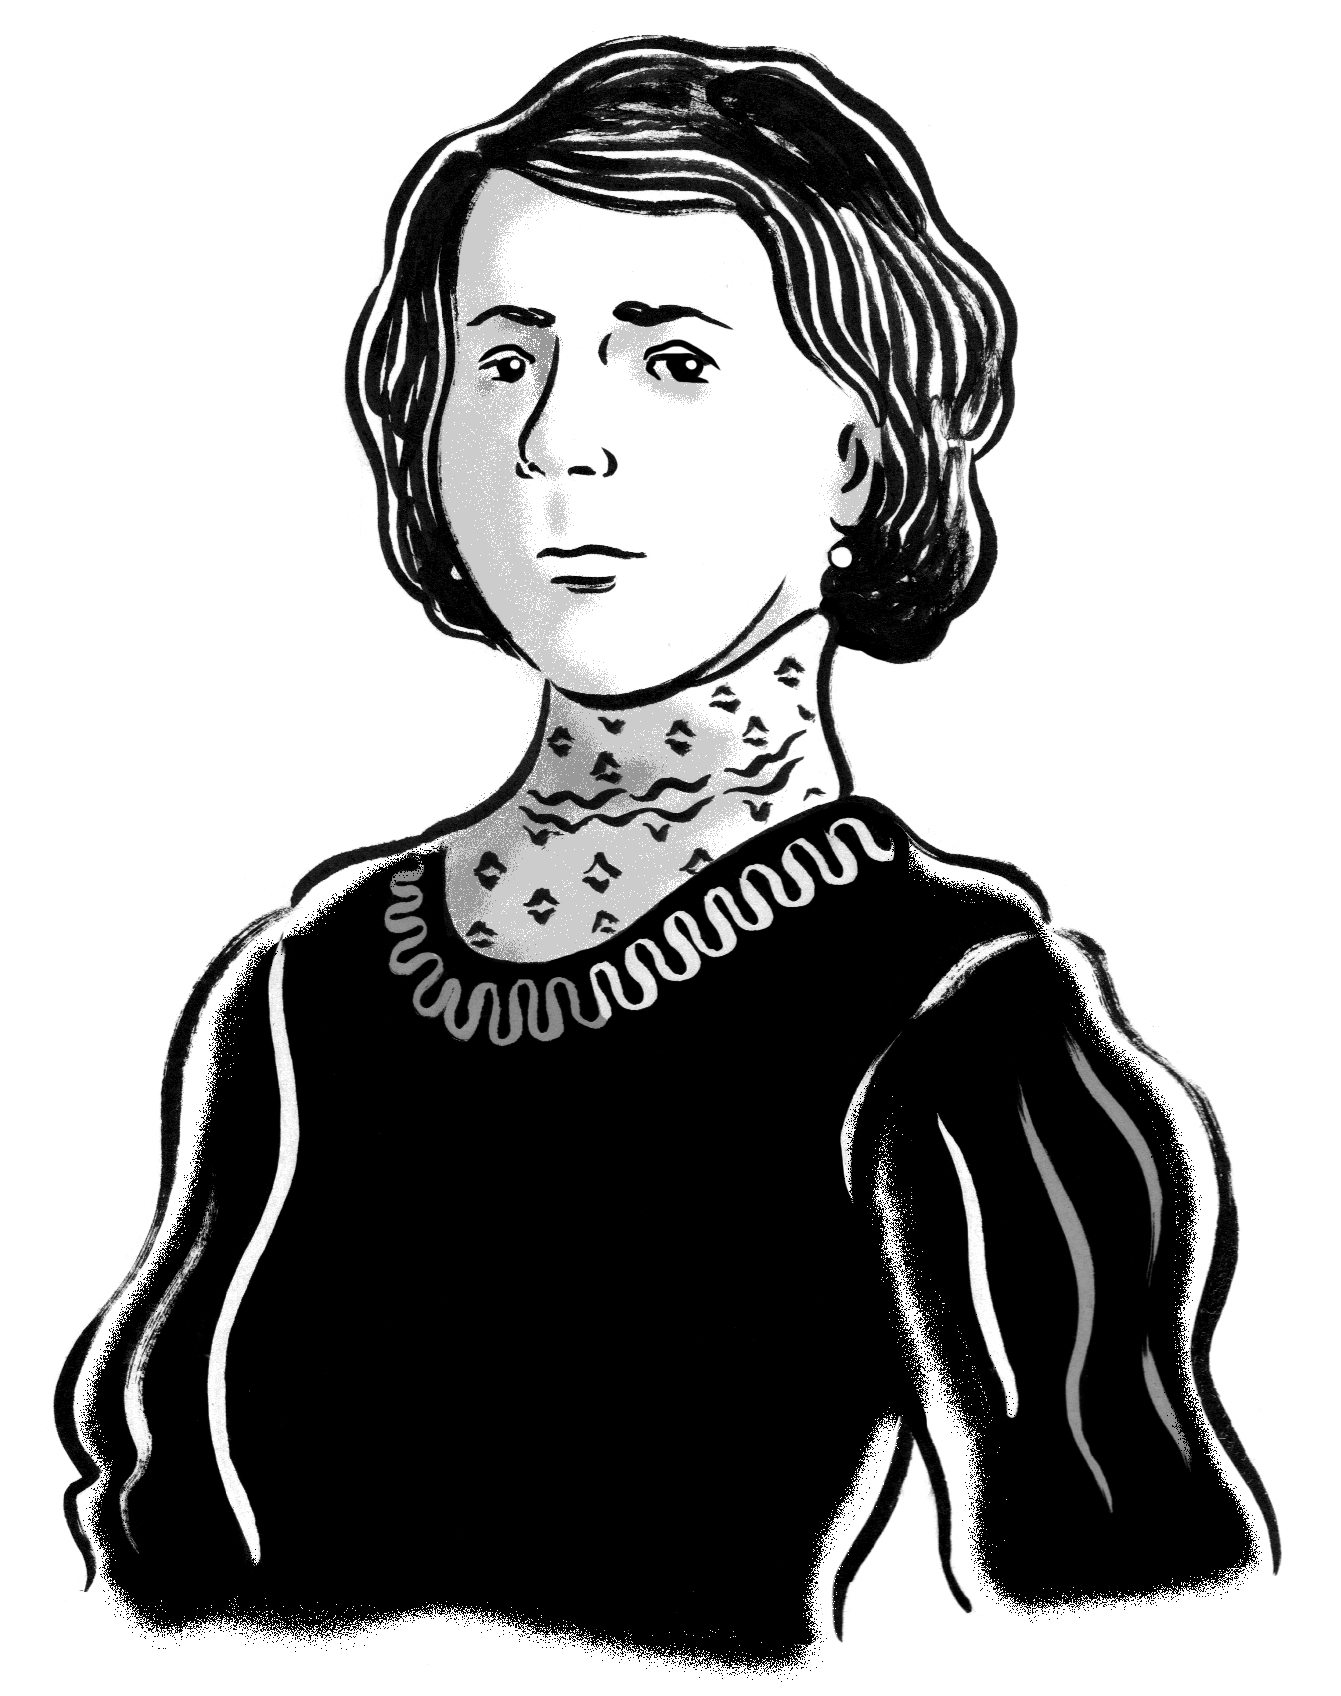
\includegraphics[width=5cm]{./images/PNLD0050-12.png}}

\paragraph{Metodologia}
São diversas as personagens femininas representadas em \emph{Contos
russos juvenis}, procedentes de épocas, camadas sociais e contextos
diversos. Apresentado o contexto da luta pela emancipação feminina
russa, é interessante sugerir aos alunos e alunas que escolham uma das
personagens para redigir uma breve análise. Tatiana, de ``Mumu'' (1854),
por exemplo, é simbólica: às portas da abolição da servidão russa, que
ocorrerá em 1861, a lavadeira surge como instrumento de ``conserto'' do
homem; ela é um semiobjeto obrigado a acatar a ordem da patroa de
colocar seu sapateiro alcoólatra na linha, estigmatizada e vítima de
preconceito supersticioso (porque tinha marcas de nascença na face
esquerda, que indicavam mau presságio), etc. Há ainda as patroas
terríveis e déspotas de ``Poodle Branco'' (1907) e ``Mumu''; mães
diversas: a ``mãe solo'' trabalhadora e viúva retratada em ``A mãe''
(1912); a que deixa o garoto no hospital em ``O fugitivo'' (1887); a mãe
cúmplice do filho em ``A pedrinha vermelha''; a mãe que negligencia o
filho em ``Primeira mágoa'' e a babá, do mesmo conto, que tinha
as funções de mãe e a quem faltava consciência de classe. Por fim, as
meninas, como a bondosa adolescente tártara, Dina, que ajuda Jílin a
fugir em ``O prisioneiro do Cáucaso'' (1872); a assustadora Zoia,
em ``A filha do fabricante de caixões'' (1918), que tenta
esfaquear o herói, o qual foge para viver; a doente Nadiejda, cujo nome,
não por acaso, significa ``esperança'' em russo, de ``O
elefante''; e a estudiosa Natália de ``A prova'' (1912).

Outra opção é trabalhar a autoria feminina. São três as autoras
representadas na coletânea: Catarina \textsc{ii}, Lídia Tcharskaia e Lídia
Avílova. Tendo em mente as biografias das escritoras e fazendo pesquisas
adicionais, o educando pode analisar os contos aqui apresentados com
base na escrita literária de autoria feminina e se perguntar: existe uma
escrita feminina? Se sim, quais seriam as características dela? A
escrita feminina poderia ser produzida por homens?


\paragraph{Tempo estimado} Três a quatro aulas de 50 minutos.

\marginnote{\footnotesize\textbf{PARA O PROFESSOR LER}\\
``Ainda sobre escrita feminina: em que consiste a diferença?''\\
\url{https://seer.ufs.br/index.php/interdisciplinar/article/view/1252/1088}
}

\subsection{Leitura}

\BNCC{EM13LP03}
\BNCC{EM13LP50}
\BNCC{EM13CHS203}

\paragraph{Tema} A relação com os animais em \emph{Contos russos juvenis}.


\paragraph{Conteúdo}
Análise da importância dada aos animais em diversas histórias de
\emph{Contos russos juvenis}.

\paragraph{Objetivos}
Levar o jovem leitor a pensar as relações da personagem com a natureza e
os animais e seu significado na obra e na vida.

\paragraph{Justificativa}
Muitas obras reunidas nesta coletânea trazem animais como protagonistas.
Não é só o caso de ``Mumu'' e ``Poodle branco, que ressaltaremos aqui,
mas também o de ``O elefante'' e de ``A pedrinha vermelha''. Além
disso, os desequilíbrios sociais, evidenciados nessas obras, algumas
vezes são apaziguados pela ternura das relações das pessoas com os
animais.

\paragraph{Metodologia}
Para realizar esta atividade, sugerimos que o professor se concentre nos
contos ``Mumu'' (1854), de Turguêniev, e ``O poodle branco''
(1907), de Kuprin, e no dialogismo e intertextualidade que permeiam as
obras. A certa altura do conto, a cachorrinha Mumu, depois de ter sido
vendida às escondidas por um criado a mando da patroa, volta para o
dono, o mudo Guerássim, com um farrapo no pescoço. É simbólica a cena em
que Mumu, ao retornar, começa a lamber Guerássim, que dormia: ``Um grito
prolongado de felicidade saiu de seu peito mudo; ele agarrou Mumu,
estreitou"-a no peito; em um instante, ela já lhe lambia o nariz, os
olhos, o bigode e a barba\ldots{}''. A cena não por acaso é retomada no fim
do conto de Kuprin, quando Artô, o \emph{poodle}, é resgatado e
reencontra seu dono dormindo, o velho tocador de realejo:

\begin{quote}
(\ldots{}) antes de ele recobrar os sentidos, o cachorro já lhe lambia, com
ganidos felizes, as faces, os olhos, o nariz e a boca. O vovô despertou,
viu a corda no pescoço do poodle, viu o menino deitado ao lado, coberto
de poeira, e compreendeu tudo. (\textsc{mountian}, 2021, p.271)
\end{quote}

O desfecho de ``Poodle branco'' é aparentemente positivo: o menino
acrobata consegue recuperar Artô, o cachorro que fora roubado da dupla
de saltimbancos pelo caseiro de uma família abastada, para satisfazer as
vontades de um menino mimado e histérico. Porém, a imagem final é
desoladora: os corpos estirados em uma taberna, que se assemelham a
cadáveres, prenunciam o difícil futuro que os saltimbancos teriam pela
frente. (\textsc{mountian}, 2021, p.363). Além disso, a clara menção ao conto de
Turguêniev (acima referida), além de prestar homenagem a um dos maiores
estilistas russos, destaca o futuro sombrio que os amigos teriam pela
frente.

\begin{figure}[ht!]
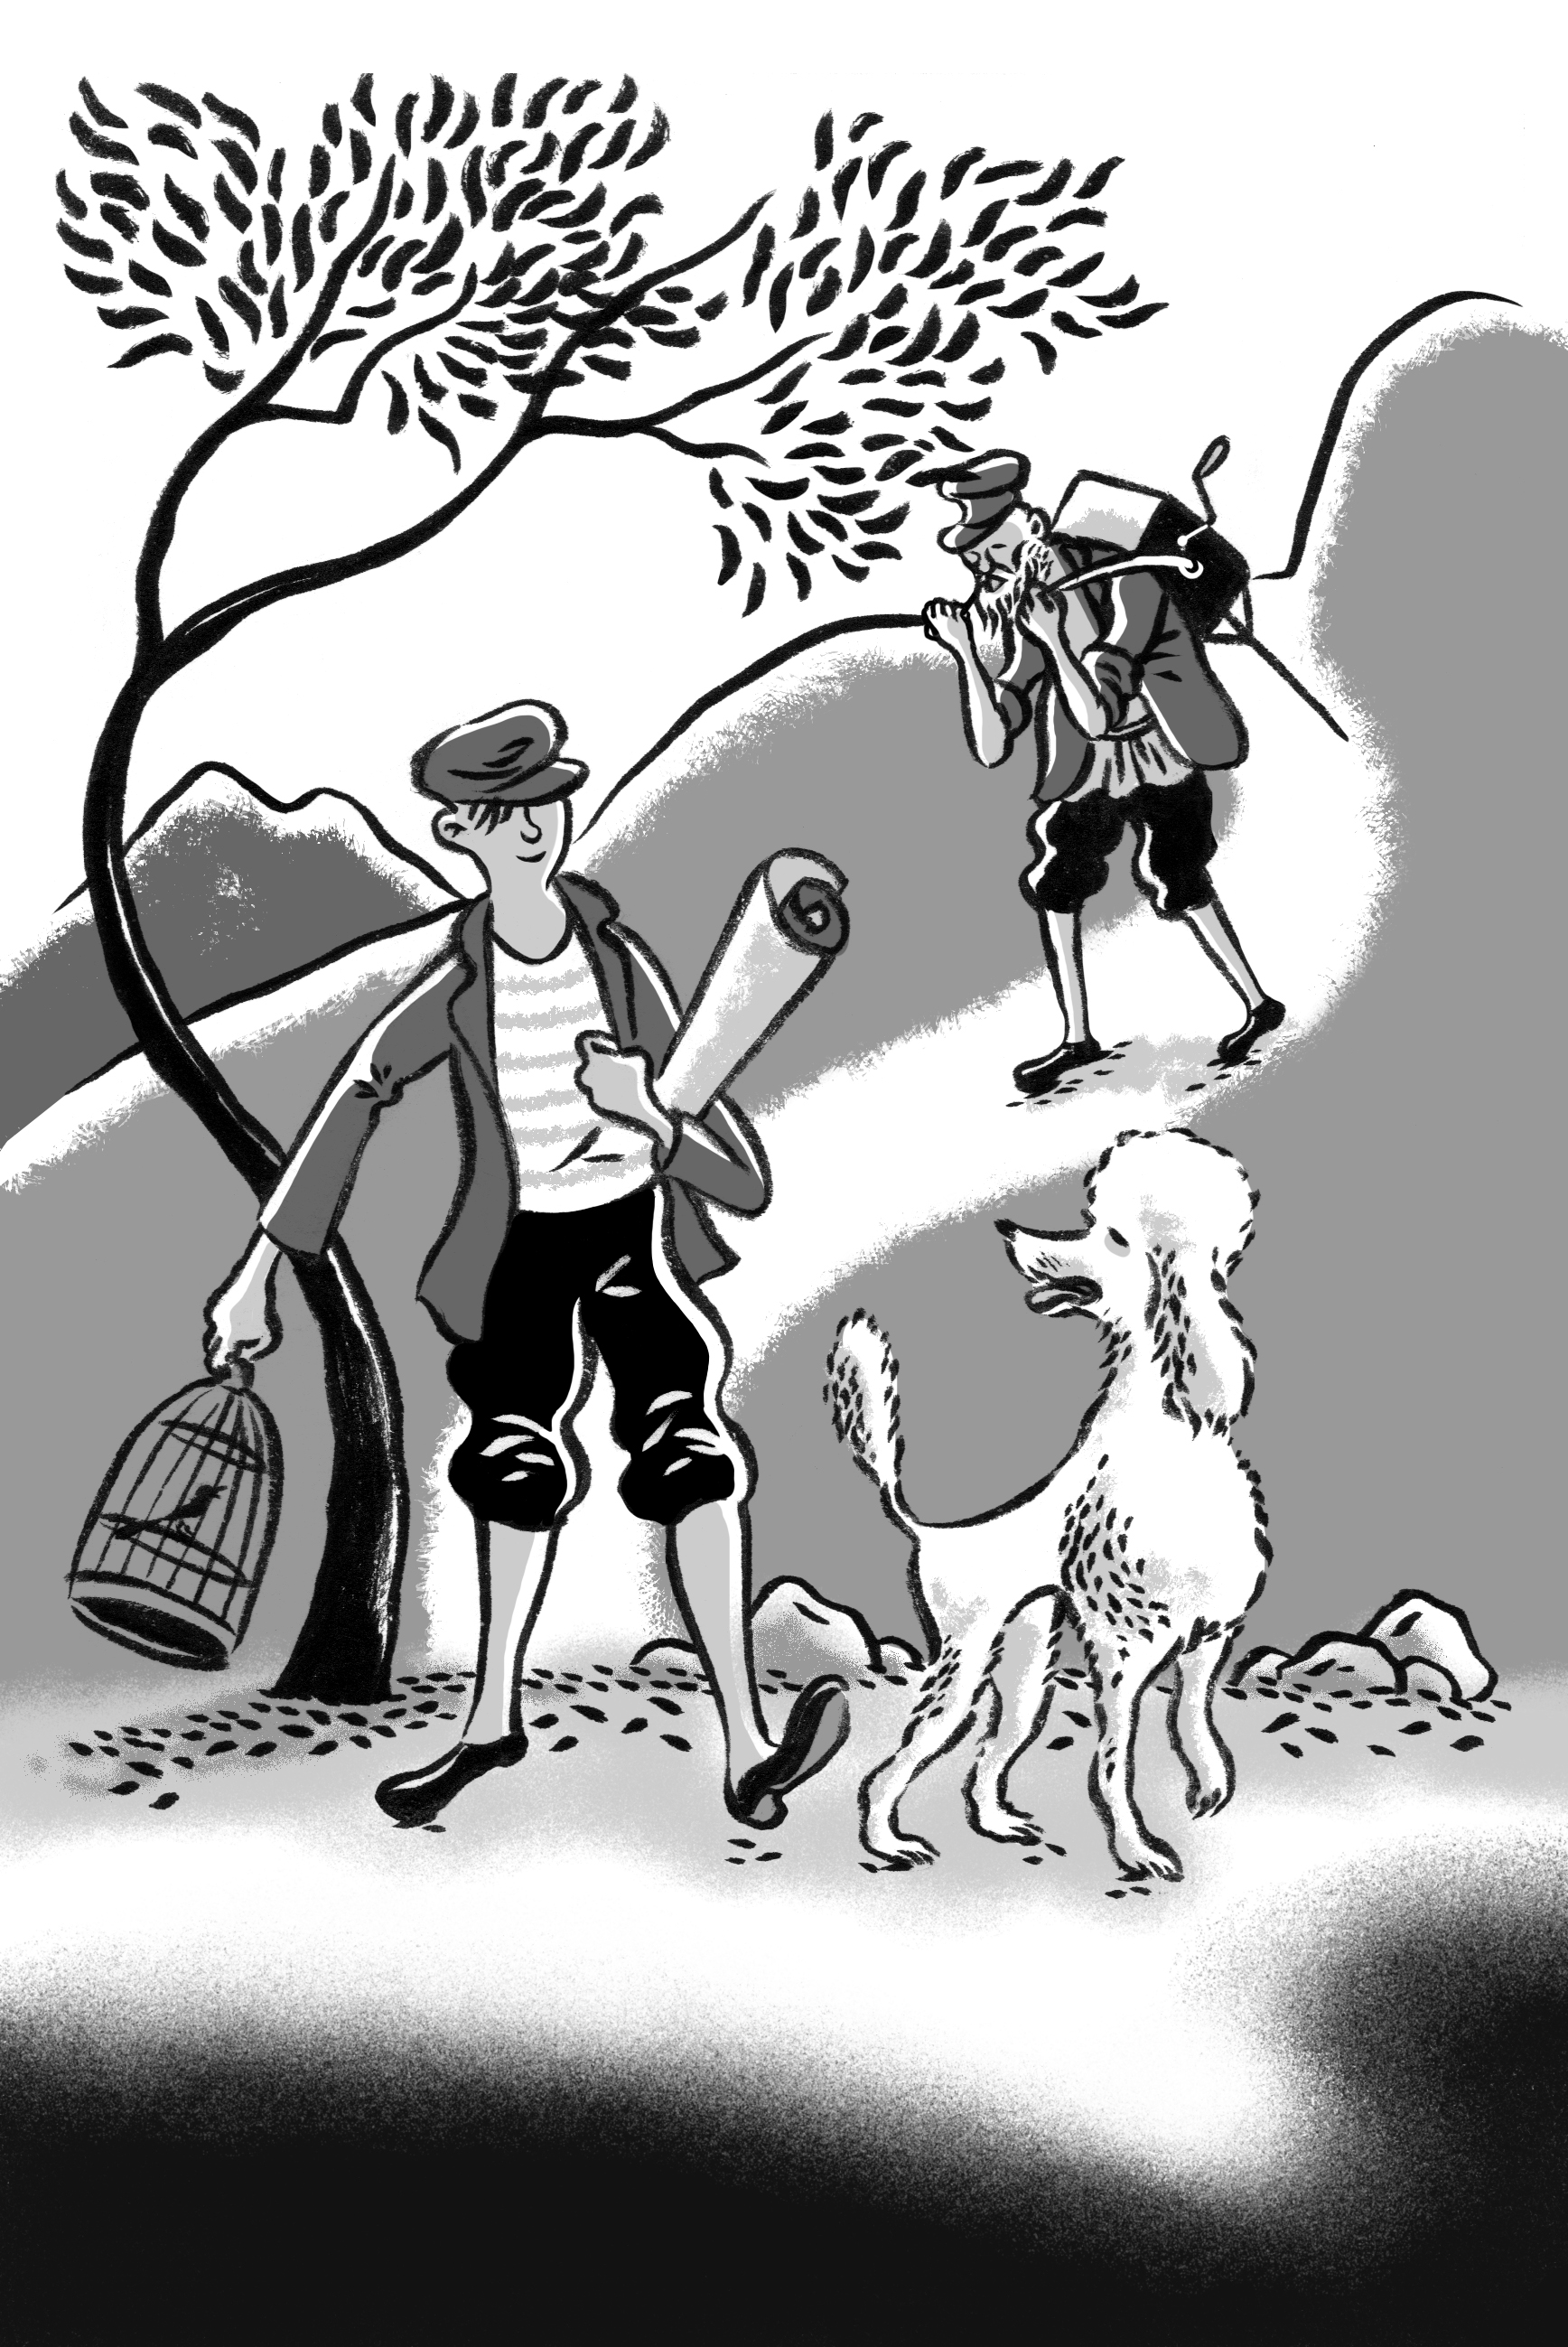
\includegraphics[width=\textwidth]{./images/PNLD0050-13.png}
\end{figure}

Turguêniev ``era filho de um nobre empobrecido que se casara por
interesse com uma rica herdeira mais velha. Teve uma infância
influenciada pela mãe, que, apesar de apegada ao filho, era despótica
com ele e cruel para com os numerosos servos''. (\textsc{bernardini}, 2018, p.
43) É interessante notar que, em ``Mumu\emph{'',} o protótipo da patroa
é a própria mãe de Turguêniev, Varvara Petrovna; e o de Guerássim, um
criado da mãe, Andrei. Mas, ao contrário de Guerássim, que faz um gesto
de protesto ao deixar a casa da patroa e voltar à aldeia, Andrei, após
ter afogado sua cachorra Mumu, fica até o fim da vida na casa da mãe de
Turguêniev.

Algumas questões podem ser colocadas ao aluno:

\begin{itemize}
\item Por que Guerássim afogou sua cachorra, a única criatura com o qual ele
tinha uma conexão depois da partida de Tatiana? Guerássim amava Mumu
perdidamente e, depois da morte dela e da partida de Tatiana, ele nunca
mais se interessou por mulheres ou por animais, ou seja, ao matar a
cadelinha, ele praticamente cometeu um suicídio\ldots{} Vale notar que há uma
aproximação da \emph{spaniel} com a criada Tatiana: Guerássim encontra a
cadela após perder o amor de sua vida.

\item Em um trecho de ``Poodle branco'', a patroa da \emph{datcha}
(espécie de chácara) luxuosa diz: ``Escute, velho insano! Não existe
coisa que não possa ser vendida''. Repensando os dois contos, o aluno
poderia escrever uma redação sobre essa frase? É verdade que tudo tem um
preço? O que o educando acha do fato de o velho saltimbanco ter se
recusado a vender o cachorro por uma soma com a qual poderia comprar uma
mercearia?

\item A intertextualidade pode se dar pelo gênero (como no texto de
Catarina, que revisita um gênero antigo), pelo tema e pelo estilo. E ela
pode ser feita via paródia ou via estilização. Como escreve Mountian
(2011, p. 54), no início do século \textsc{xx}, Iúri Tyniánov, um teórico russo,
inovou a compreensão do elemento paródico:

\begin{quote}
Tyniánov {[}\ldots{}{]} pode ser considerado o precursor dessa abordagem,
levando a \emph{paródia} no contraste com a \emph{estilização}. Tanto a
paródia como a estilização inserem outra fala na obra, mas na paródia
está sempre implícito um conflito, um embate, enquanto na estilização há
um prosseguimento. A paródia estabelece um deslocamento, que dá à fala
original outra função, produzindo uma inversão do discurso. A essência
da paródia não é definida pelo cômico, mas pela descontinuidade de dois
planos.
\end{quote}

No caso apontado, a intertextualidade se dá por estilização e sobretudo
no campo temático: a relação afetiva de pessoas desprovidas de tudo (o
caseiro Guerássim e o tocador de realejo Lodýjkin) com os cães, a ameaça
de perda --- o sacrifício do animal, em um caso, e a recuperação dele,
em outro. O aluno consegue estabelecer outras relações intertextuais
entre esses dois contos da coletânea? Como a questão da orfandade é
tratada em ``Poodle branco'' e ``Vanka''? Em ``Primeira mágoa'' e
``Poodle branco'' surge a questão da ausência de documentos: como a
falta deles influencia o destino das personagens?
\end{itemize}

\paragraph{Tempo estimado} Três a quatro aulas de 50 minutos.

\subsection{Pós"-leitura}

\BNCC{EM13LP14}
\BNCC{EM13LP50}

\paragraph{Tema} ``A alma do conto em uma imagem'': a leitura paratextual de \emph{Contos russos juvenis}.


\paragraph{Conteúdo}
Análise das ilustrações e dos elementos gráficos da coletânea em sala de aula.

\paragraph{Objetivos}
Apresentar os diversos sentidos das ilustrações, explorar os paratextos
como elementos compositivos do livro e desenvolver um projeto que amplie
a experiência literária juvenil.

\paragraph{Justificativa}
Para um trabalho eficiente com a literatura infantil e juvenil, é
preciso apresentar os diversos sentidos das ilustrações, explorar os
paratextos como elementos compositivos do livro como objeto e criar um
projeto que amplie e emancipe a experiência literária dos jovens
leitores, conforme apontam Camargo (1998), Colomer (2007) e Lins (2003)
(\emph{apud} \textsc{pontes}, \textsc{betta}, 2020, p.128). Além disso, como escreve
Pelegrini (2003 \emph{apud} \textsc{betta}, \textsc{pontes}, 2020, p. 130), a sociedade
contemporânea é midiatizada por imagens: ``a cultura contemporânea é
sobretudo visual. Videogames, videoclipes, cinema, telenovela,
propaganda e história em quadrinhos são técnicas de comunicação e de
transmissão de cultura cuja força retórica reside sobretudo na imagem''.

Assim, o exercício de análise de imagens é uma atividade de grande
relevância no processo de construção e estabelecimento de conhecimento:
``Didi"-Huberman sugere que a imagem seja feita não só de sentidos, mas
também de sintomas (uma ruptura dentro do saber) e conhecimento (ruptura
dentro do caos), levando a inquietações do pensamento''. (\textsc{reis}, 2013 p. 1)

Este trabalho com os educandos evidenciará a importância das imagens e
dos paratextos no livro, ampliando e qualificando o processo de leitura
literária e proporcionando a oportunidade de o educando desenvolver sua
sensibilidade ao consumir essas produções e realizar conexões.

\paragraph{Metodologia}
Nesta atividade, os alunos terão a oportunidade de explorar as imagens
do ilustrador Fido Nesti. Nascido em São Paulo, em 1971, Nesti produz
ilustrações para capas, livros e quadrinhos há mais de trinta anos,
tendo publicado sua obra também no jornal \emph{Folha de S.Paulo} e na
revista \emph{The New Yorker}, com a qual colaborou por quase dez anos,
entre outros veículos.

A educação imagética e paratextual da literatura no contexto escolar
pode trabalhar os diversos sentidos da imagem (que pode ser
representativa, descritiva, narrativa, simbólica, expressiva, estética,
lúdica, conativa, metalinguística ou fática) e buscar a valorização dos
paratextos. Formato, título, capa: tudo pode e deve ser explorado
durante a leitura. Isso tudo contribui para a formação dos leitores,
aguçando seu olhar:

\begin{quote}
A leitura dos paratextos constitui o primeiro contato do leitor com o
material escrito e, dessa maneira, pode servir como um ``guia de
leitura'', pois a compreensão dos paratextos antecipa questões que podem
ser respondidas quando a criança entrar no livro e começar a lê"-lo.
(\textsc{silva}; \textsc{souza}, 2016, p. 79; apud \textsc{betta}, \textsc{pontes}, 2010, p. 132)
\end{quote}

As ilustrações de Fido, de traço forte, estão inseridas na
contemporaneidade por dialogarem com \textsc{hq}, universo muito atraente para o
público juvenil. Ao mesmo tempo, elas refletem minuciosamente os
costumes, trajes e cenários descritos ou deduzidos dos contos da
coletânea. Quanto à relação com \textsc{hq}, Fido lembra que é espontânea:

\begin{quote}
É natural, porque trabalho muito com \textsc{hq}. Boa parte da minha carreira foi
voltada para ilustrações, mas intercalada com \textsc{hq}s. E depois dessa
revolução tecnológica, com o fechamento de muitas revistas, a \textsc{hq} ganhou
mais espaço no meu trabalho. Meu traço tem um quê de \emph{cartunesco},
como se costuma falar, e fica no meio termo entre algo mais, talvez,
realista e artístico, com um quê de quadrinho, pois gosto de dosar
também. (\textsc{nesti}, 2021)
\end{quote}

Ramos e Nunes (2013 apud \textsc{betta}, \textsc{pontes}) descrevem o papel de uma
ilustração bem elaborada como de ``abrir frestas'' na história,
tornando"-se atrativos visuais que fazem o leitor ``mergulhar'' nela. Com
um traçado preciso feito a nanquim, que é posteriormente tonalizado no
computador, as imagens de Fido também são dotadas de grande
expressividade:

\begin{quote}
Acho muito importante na formação infantojuvenil as referências
pictóricas que o leitor tem nas primeiras leituras. Eu guardo na memória
até hoje as imagens dos livros que eu tinha quando criança, por isso
tenho sempre esse cuidado e capricho no desenho e em tentar traduzir a
minha visão do texto sintetizando os detalhes. Eu busco ir atrás da alma
do conto em uma imagem. (\textsc{nesti}, 2021)
\end{quote}

Para elaborar as imagens para \emph{Contos russos juvenis,} Fido
realizou uma extensa pesquisa, envolvendo não apenas os períodos
tratados na obra, como detalhes dos diferentes povos retratados. Isso
pode ser percebido, por exemplo, nas vestes de Dina, a moça tártara que
ajuda Jílin a fugir em ``O prisioneiro do Cáucaso'', ou na gaita
de fole que surge no conto de Catarina \textsc{ii}, uma versão regional russa
antiga que é mais rudimentar, composta por um saco de couro com três
aberturas. A \emph{datcha} de ``A pedrinha vermelha'' também foi
minuciosamente pesquisada para compor o plano de fundo da imagem. Assim,
cada uniforme, cada capacete, cada detalhe foi estudado pelo artista. A
apresentação teórica irá surpreender os alunos pela profundidade e pelo
trajeto necessário para se desenvolver a narrativa visual dos livros
infantojuvenis.

\begin{figure}[ht!]
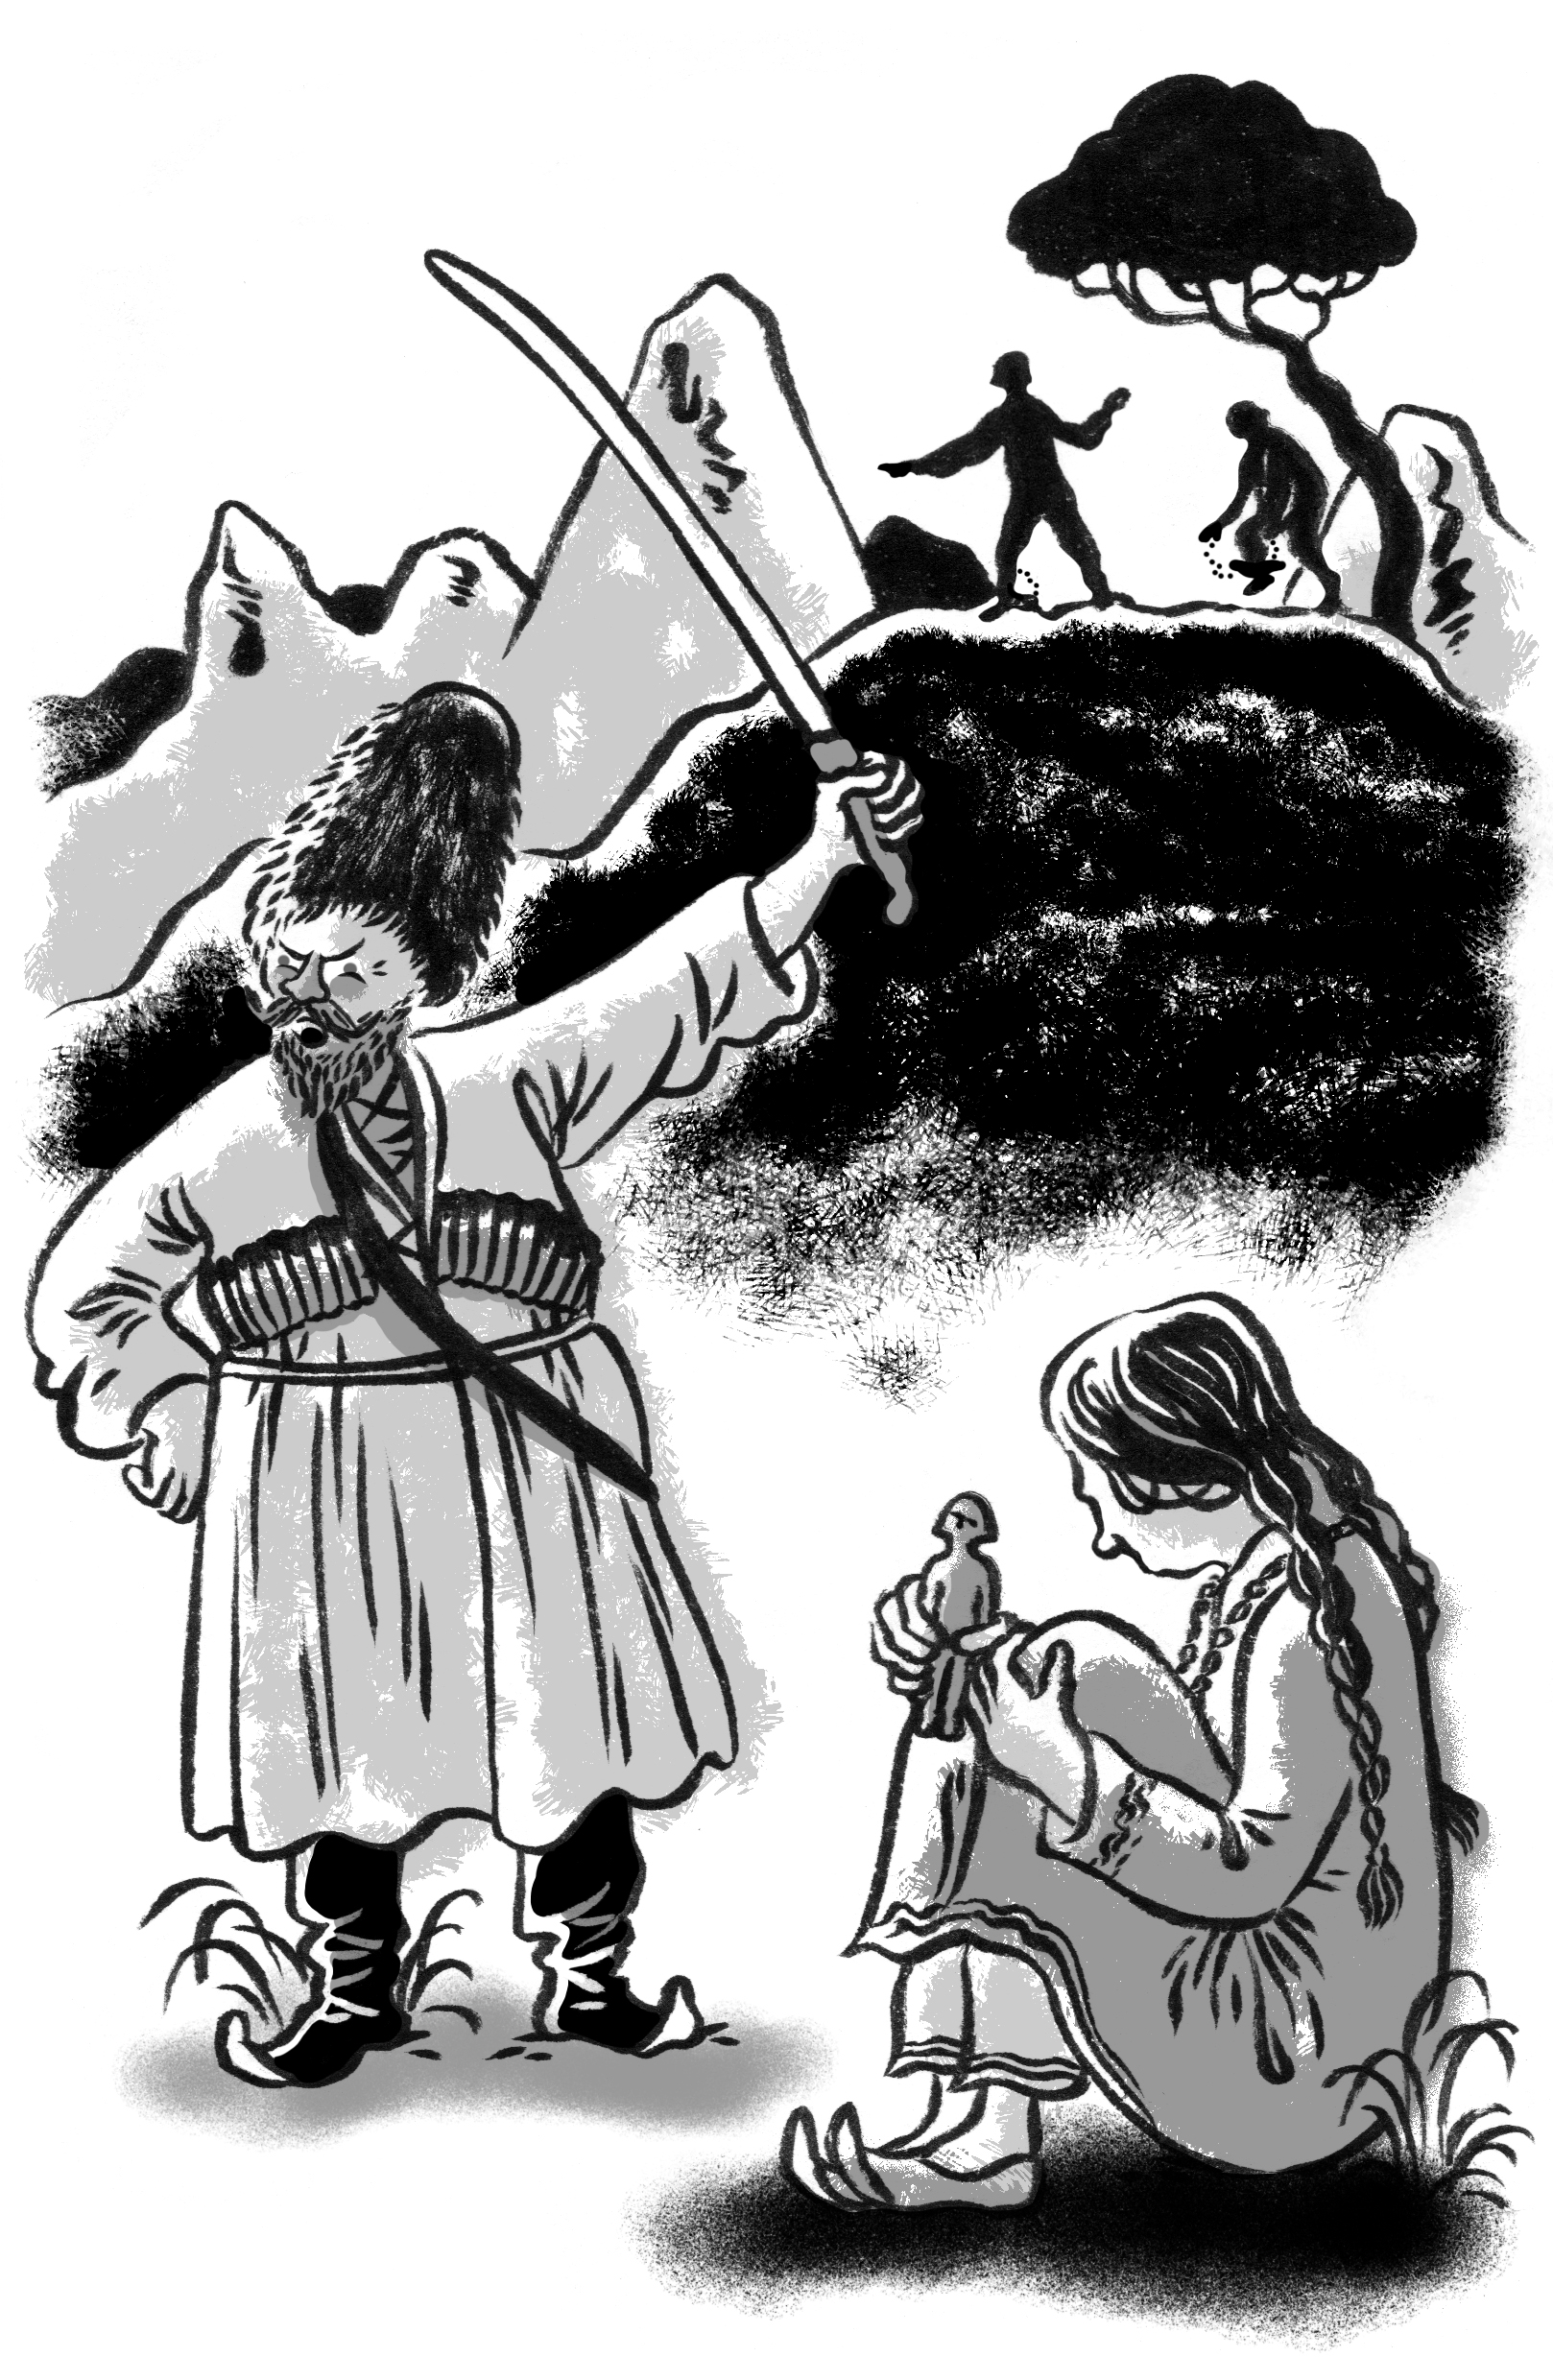
\includegraphics[width=\textwidth]{./images/PNLD0050-14.png}
\end{figure}

Como primeiro passo para a análise das imagens pelos alunos, sugerimos
que o educador apresente algumas funções inerentes a elas, conforme a
proposição de Camargo (1998 apud \textsc{betta}, \textsc{pontes}): representativa,
descritiva, narrativa, simbólica, expressiva, estética, lúdica,
conativa, metalinguística, fática e pontuação. \emph{Contos russos
juvenis} traz na capa, por exemplo, um espelhamento de um menino num
velho, que mostra o início e o fim da vida, numa cena inspirada na
ilustração do conto ``O fugitivo'' (1887), de Tchékhov.

Os alunos podem tentar localizar as cenas desenhadas nos contos,
discuti"-las, selecionar suas ilustrações prediletas, desenhar outras e
compartilhar com a classe suas impressões. Para que a proposta não
intimide os estudantes menos interessados no desenho, pode"-se sugerir
que as ilustrações sejam experimentais e que tenham o texto apenas como
ponto de partida --- afinal, a atividade não tem como finalidade avaliar
as habilidades técnicas do educando, mas colocá"-lo diante da construção
de uma narrativa visual, o que lhe dará uma nova experiência com o texto
literário.

\paragraph{Tempo estimado} Duas aulas de 50 minutos.


\section{Referências bibliográficas}

\begin{itemize}
\item[]\textsc{bernardini}, Aurora Fornoni. \emph{Aulas de Literatura Russa.}
São Paulo: Kalinka, 2018.

\item[]\textsc{betta}, Thiago; \textsc{pontes}, Rodolfo. \emph{A ilustração do conto infantil:
uma proposta para a educação literária imagética e paratextual na sala
de aula}. Literartes, n° 13, 2020, p.128-149

\item[]\textsc{bosi}, Alfredo. ``Situação e forma do conto brasileiro contemporâneo''.
In: \emph{O conto brasileiro contemporâneo}. São Paulo: Cultrix, 1977.

\item[]\textsc{cortázar}, Julio. \emph{Valise de cronópio}. São Paulo: Perspectiva, 1993

\item[]\textsc{goldman}, Wendy. \emph{Mulher, Estado e Revolução}. São Paulo: Boitempo,
2014.

\item[]\emph{Catarina, a Grande} (Philip Martin, 2019, disponível no \textsc{hbo go}).\\
\textsc{kersley}, Sarah Rebbeca. \emph{Quatro poemas de Sérgio Capparelli}.
Cadernos de Literatura em Tradução, n°12, 2011.

\item[]\textsc{lear}, Edward. \emph{Conversando com varejeiras azuis}. São Paulo:
Iluminuras, 2016

\item[]\emph{Mágico de Oz, O.} Direção: Fleming, Victor. Estados Unidos: Loews,
1939.

\item[]\textsc{márquez}, Gabriel García. \emph{Como contar um conto}. Rio de Janeiro:
Casa Jorge Editorial, 2004.

\item[]\textsc{moisés}, Massaud. \emph{A criação literária.} São Paulo: Cultrix, 2001

\item[]\textsc{moisés}, Massaud. \emph{Dicionário de termos literários}. São Paulo:
Cultrix, 2004

\item[]\textsc{mountian}, Daniela (Org.). \emph{Contos russos juvenis.} São Paulo:
Kalinka, 2021.

\item[]\textsc{mountian}, Daniela. Prefácio. Paratexto. \emph{Contos russos juvenis.}
São Paulo: Kalinka, 2021.

\item[]\textsc{mountian}, Daniela. \emph{A vanguarda dos livros russos infantis}. Curso
de inverno. \textsc{usp}/2020. Canal de Serviço de Cultura e Extensão \textsc{fflch}/\textsc{usp}):
\url{https://www.youtube.com/watch?v=2l4v9rkW6H4}

\item[]\textsc{nesti}, Fido. Entrevista telefônica concedida à Editora Kalinka para o
Manual do Professor de \emph{Contos Infantojuvenis Russos} em
10/02/2021.

\item[]\textsc{paixão}, Biana Alves da. \emph{A literatura infantil de Daniil Kharms:
tradição e modernidade}. Dissertação de mestrado. Universidade de São
Paulo, 2015.

\item[]\emph{Prisioneiro das Montanhas}. Direção: Bodrov, Serguei. Rússia,
Cazaquistão: \textsc{ao} Karavan, \textsc{bg}g Prodakchn, 1996.

\item[]\textsc{reis}, Ana Paola dos. A análise de imagens como método de pesquisa e
recurso didático. Conferência Fido Palermo 2013.
Disponível em:
\url{https://fido.palermo.edu/servicios_dyc/encuentro2010/administracion-concursos/archivos_conf_2013/1131_85939_1689con.pdf}

\item[]\textsc{soares}, Angélica. \emph{Gêneros Literários}. São Paulo: Ática, 2007.

\item[]\textsc{urso}, Graziela Schneider (org.). \emph{A revolução das mulheres}. São
Paulo: Boitempo, 2002.

\item[]\textsc{woolf}, Virginia. \emph{Um teto todo seu.} São Paulo: Tordesilhas, 2017.
\end{itemize}

\section{Sugestão de bibliografia comentada}

\subsection{Sobre o conto como gênero}

\begin{itemize}
\item\textsc{andrade}, Mário. de. ``Contos e contistas'' \textsc{in}: \emph{O empalhador de
passarinho}. 3 ed. Brasília: \textsc{inl}, 1972, p. 5-8.

Escrito a propósito
de uma pesquisa da \emph{Revista Acadêmica} que procurava determinar os
dez melhores contos brasileiros; o artigo discute a questão do gênero.

\item\textsc{benjamin}, Walter. ``O narrador: considerações sobre a obra de Nikolai
Leskov''. In: \emph{Walter Benjamin: magia e técnica, arte e política}.
São Paulo: Brasiliense, 3ª ed., 1985.

Benjamin nota que o jornal vem
cheio de informações e, portanto, não existe mais narrador para ele ---
de certa forma, a informação mata a narrativa da experiência ---, e que
Leskóv é do tempo em que a narrativa da experiência importa. Assim,
segundo Benjamin, Leskóv dialoga com seus leitores, que são praticamente
ouvintes, e a narrativa é inesgotável, sempre mais interpretável que a
informação.

\item\textsc{cortázar}, Julio. ``Alguns aspectos do conto''; ``Do conto breve e seus arredores'' e ``Poe: o poeta, o narrador e o crítico''. In: \emph{Valise
de cronópio}. São Paulo: Perspectiva, 1993, p.147-163, p. 227-237 e
103-146. 

``Alguns aspectos do conto'' é resultado de uma conferência
feita aos cubanos, em 1963, e trata de questões referentes aos contos de
Cortázar e aos contos em geral, buscando acompanhar o processo da
criação, analisando a peculiaridade do gênero e questionando o caráter
revolucionário dos escritores. ``Do conto breve e seus arredores'' parte
de uma afirmação de Quiroga para discutir a esfericidade do conto, suas
relações com a poesia e prosa, além de tecer considerações sobre o conto
fantástico. ``Poe: o poeta, o narrador e o crítico'' é um texto que
examina com consciência e entusiasmo a obra de Poe e acompanha a
tradução de sua obra para o espanhol feita por Cortázar.

\item\textsc{gotlib}, Nadia. \emph{Teoria do conto}. São Paulo: Ática, 2006.

A autora situa o conto enquanto narrativa, discutindo"-o enquanto um
``gênero'' com características próprias, relatando também seu percurso, de
suas origens remotas e anônimas até sua afirmação com autoria literária.

\item\textsc{jolles}, André. \emph{Formas simples}. Trad. de Álvaro Cabral. São Paulo,
Cultrix, 1976. 

Este livro examina o conto como forma simples, ao
lado de outras (como legenda, saga, mito, adivinha, ditado, caso,
memorável, chiste), traçando diferenças quanto à forma artística.

\item\textsc{poe}, Edgar Allan. ``Filosofia da composição''. In: \emph{Ficção
completa, poesia \& ensaios}. Org., trad. e notas por Oscar Mendes, em
colaboração com Milton Amado. Rio de Janeiro, Aguilar, 1981. p. 11-20.


Neste texto, Poe reforça sua teoria da unidade de efeito e os modos
de se obter essa unidade, explicitando seu processo consciente de
composição.

\item\textsc{tchékhov}, Anton. \emph{Sem trama e sem final: 99 conselhos de escrita}.
São Paulo: Martins Fontes, 2007. Organização: Homero Freitas de Andrade.
\end{itemize}

\end{document}


